\documentclass[12pt %
,a4paper %
,titlepage %
,twoside %
%,openany % ouvre les sections indifféremment sur la page de gauche ou de droite
]{book}

%\usepackage{layout}
%\usepackage[nomarginpar, margin=3cm]{geometry}
% Paramétrages de la langue et de l'encodage
\usepackage[utf8]{inputenc}
\usepackage[frenchb]{babel}
\usepackage[T1]{fontenc}

% formules mathématiques
\usepackage{amsmath}
\usepackage{amsfonts}
\usepackage{amssymb}

% gestion des graphiques
\usepackage{graphicx}

% Gestion des couleurs
\usepackage[usenames,dvipsnames]{xcolor}

% Redefinition des liens web
\usepackage{url}
\usepackage[colorlinks=false,urlbordercolor=white,linkbordercolor=white]{hyperref}

% Définition des marges de la page
%\usepackage[left=2cm,right=2cm,top=2cm,bottom=2cm]{geometry}

% Polices de caractères
\usepackage{lmodern}
\usepackage{mathptmx} % times, y compris dans les formules mathématiques

% Insertion de code source dans le texte, à utiliser avec \begin{lstlisting} et \lstset{java|html|php...}
\usepackage{listingsutf8}

% Definition de l'affichage du code
\lstset %
{
basicstyle=\ttfamily\small, %frame=single %
,showstringspaces=false %
,tabsize=2 %
,breaklines=true, %
,inputencoding=utf8/latin1 %
,literate=
    {é}{{\'e}}{1}%
    {è}{{\`e}}{1}%
    {à}{{\`a}}{1}%
    {â}{{\^a}}{1}%%%
    {ç}{{\c{c}}}{1}%
    {œ}{{\oe}}{1}%
    {ù}{{\`u}}{1}%
    {É}{{\'E}}{1}%
    {È}{{\`E}}{1}%
    {À}{{\`A}}{1}%
    {Ç}{{\c{C}}}{1}%
    {Œ}{{\OE}}{1}%
    {Ê}{{\^E}}{1}%
    {ê}{{\^e}}{1}%
    {î}{{\^i}}{1}%
     {ï}{{\"i}}{1}%%%
    {ô}{{\^o}}{1}%
    {û}{{\^u}}{1}%
}

% Définition des entêtes
\usepackage{fancyhdr}
\pagestyle{fancy}

% Redéfinition des titres de section
\usepackage{titlesec}

% Insertion de graphiques à des emplacements définis
\usepackage[abs]{overpic}

% Tableaux
\usepackage{array}
\usepackage{longtable}
\usepackage{float}

% règles typographiques de l'Imprimerie nationale
\usepackage[all]{nowidow}
\usepackage[
% frenchchapters renomme le premier chapitre, mais :
%	- cela pose problème dans la table des matières
%	- cela ne peut être utilisé qu'avec la renumérotation des chapitres activée
%frenchchapters,
parindent,
lastparline,
hyphenation
]{impnattypo}

% Renumérotation des chapitres
%\renewcommand{\thesection}{\Alph{section})}
%\renewcommand{\thesubsection}{\arabic{subsection} -}
%\renewcommand{\thesubsubsection}{\alph{subsubsection} -}
%\usepackage{engrec}
%\renewcommand{\theparagraph}{\engrec{paragraph})}
%\setcounter{secnumdepth}{4}

% Génération du code Ipsum lorem
%\usepackage{blindtext}



% Definition des couleurs IRSTEA
%\definecolor{titreColor}{RGB}{0,58,128}  % Marine
%\definecolor{stitreColor}{RGB}{0,158,224}  % Ocean
%\definecolor{auteurColor}{RGB}{0,58,128}     % Marine
%\definecolor{texteColor}{RGB}{164,196,0}     % Prairie

% Definition des chapitres
\titleformat{\chapter}[display]
{\normalfont\Large\filcenter\sffamily}{
 %\MakeUppercase{\chaptertitlename}
 \chaptertitlename~\thechapter}
{1pc}
%{\titlerule
%% \vspace{1pc}%
\Large

\titleformat{\section}
{\normalfont\Large\bfseries\sffamily}
{\thesection}{1em}{}

\titleformat{\subsection}
{\bfseries\sffamily}
{\thesubsection}{1em}{}

\titleformat{\subsubsection}
{\sffamily\itshape}
{\thesubsubsection}{1em}{}


% Bibliographie
% natbib est indispensable si la biblio contient des accents
% Options pour natbib (extrait de http://merkel.zoneo.net/Latex/natbib.php)
%    round: (par défaut) pour des parenthèses arondies (());
%    square: pour des crochets ([]);
%    curly: pour des accolades ({});
%    angle: pour des équerres (<>) ;
%    colon: (par défaut) pour séparer les citations multiples par deux points (:);
%    comma: pour utiliser une virgule comme séparateur;
%    authoryear: (par défaut) pour des citations auteurs-année;
%    numbers: pour des citations numériques;
%    super: pour des citations numériques en exposant, comme dans Nature;
%    sort: ordonne les citations multiples dans l'ordre dans lequel elles apparaissent dans la bibliographie;
%    sort&compress: comme sort mais en plus les citations numériques multiples sont comprimées, si possible (3-6, 15, par exemple);
%    longnamesfirst: transforme la première citation à une référence en une version étoilée (avec la liste complète des auteurs) et le citations suivantes normales (liste abbrégée);
%    sectionbib: pour redéfinir \thebibliography pour avoir une \section* à la place d'un \chapter*; valide seulement pour les classes de document possédant la commande \chapter; à utiliser avec le paquetage  chapterbib;
%    nonamebreak: garde tous les noms d'auteurs d'une citation sur une même ligne; celà cause des problèmes de débordement, mais permet de résoudre certains problèmes liés à hyperref.

% En cas de souci, supprimez les fichiers .aux et .bbi après modification des paramètres
\usepackage[square,sort,comma,numbers]{natbib}
% styles natbib natifs : abbrvnat, plainnat, unsrtnat
\bibliographystyle{unsrtnat}
\usepackage{hypernat}
% Ajout de la référence à la bibliographie dans la table des matières
\usepackage[nottoc, notlof, notlot]{tocbibind}

\usepackage{titling}
\newcommand{\subtitle}[1]{%
  \posttitle{%
    \par\end{center}
    \begin{center}\large#1\end{center}
    \vskip0.5em}%
}

%Données de titre et d'auteur pour la page de garde
\newcommand{\titre}{Framework PrototypePHP}
\newcommand{\sousTitre}{Documentation générale - version 3.4.0}
\newcommand{\auteur}{Éric Quinton}
\newcommand{\dateModif}{\today}
\title{\titre}
\subtitle{\sousTitre}
\author{\auteur}
\begin{document}
%\layout
%Supprime les veuves et orphelines
\widowpenalty=10000
\clubpenalty=10000
\raggedbottom 
\maketitle
% Integrer la page de garde

% Définition des entêtes
\fancyhead{}
\fancyhead[CO]{\leftmark\sffamily}
\fancyhead[CE]{ \sffamily\titre{}}
\fancyfoot[CO]{\sffamily\thepage}
\fancyfoot[CE]{\sffamily\thepage}
% Redéfinition de \cleardoublepage pour créer une page totalement vide
%\makeatletter
%\def\cleardoublepage{\clearpage\if@twoside \ifodd\c@page\else
%  \hbox{}
%  \vspace*{\fill}
%
%  \vspace{\fill}
%  \thispagestyle{empty}
%  \newpage
%  \if@twocolumn\hbox{}\newpage\fi\fi\fi}
%\makeatother

\tableofcontents

\frontmatter
% \cleardoublepage permet de générer une page vide 
% si le chapitre ne commence pas sur la page de droite
% Table des matières

% Ajout d'un préambule

%\cleardoublepage
\mainmatter

\chapter{Présentation}
\section{Historique}
Au début des années 2000, PHP commençait à être largement utilisé pour créer des applications web. Certains frameworks étaient déjà présents, mais ils présentaient souvent des difficultés pour les appréhender et n'étaient pas forcément adaptés aux besoins de l'époque (performance souvent insuffisante en raison d'un chargement systématique de toutes les classes, fonctionnement exclusivement objet, etc.). De plus, ils ne permettaient que difficilement de remplacer certains composants par d'autres.

Des outils comme Smarty, un moteur de templates qui permet de séparer le code HTML du code PHP commençaient à se faire une place. On trouvait également des bibliothèques assez élaborées comme PHPGACL pour gérer les droits de manière particulièrement pertinente.

La gestion des bases de données n'était pas des plus optimales, et un souvent un peu trop conceptuelle.

PrototypePHP a été créé pour assembler divers outils disponibles, selon la con-ception qu'en avait l'auteur à l'époque. Il était loin d'être parfait et a évolué de multiples fois, pour intégrer une approche mvc, puis des contraintes de sécurité, etc. Toutefois, les fondements de départ sont restés quasiment identiques, même si certaines évolutions ont été intégrées :
\begin{itemize}
\item des actions décrites dans un fichier xml, qui est utilisé pour générer le menu en fonction des droits détenus par l'utilisateur ;
\item une gestion des droits basée sur PHPGACL. Si le produit initial a été abandonné, sa philosophie a été conservée ;
\item une séparation du code PHP et HTML avec l'utilisation de SMARTY ;
\item un accès aux tables de la base de données réalisé par l'intermédiaire d'une classe dédiée à cet usage, ObjetBDD, qui contient des fonctions très simples à manipuler, comme ecrire(\$data), lire(\$id), supprimer(\$id). La connexion à la base de données, à l'époque réalisée en utilisant la bibliothèque ADODB, a été remplacée par PDO ;
\item un support de l'identification selon quatre modalités : base de données, annuaire LDAP, annuaire LDAP puis base de données, et connexion via un serveur CAS ;
\item un souci permanent de la performance, lié au passé de son concepteur\footnote{il a commencé sa carrière à une époque où les ressources informatiques étaient rares, chères, et dont la puissance était limitée}.
\end{itemize}

La première version publiée l'a été en 2008, dans sourceforge \\ (\url{https://sourceforge.net/projects/prototypephp/}). Depuis quelques années, elle est disponible dans github \\(\url{https://github.com/equinton/prototypephp}), la branche active étant la branche \textit{bootstrap}, créée au moment du basculement de l'affichage en utilisant les fonctionnalités de ce produit.

Si le principe général d'une conception MVC a prévalu depuis plusieurs années, des améliorations récentes, notamment dans la gestion des vues, a été apportée. À partir de septembre 2016, une meilleure gestion des droits a été implémentée, notamment dans les contextes de travail avec un annuaire d'entreprise LDAP. 
Il n'est pas impossible également que le support de Shibboleth puisse être intégré dans le futur, notamment quand des bibliothèques prêtes à l'emploi seront disponibles.

\section{Gestion des versions}

Le framework est mis à jour en parallèle aux développements de logiciels bâtis à partir de celui-ci. Le code disponible reflète donc les retranscriptions des modifications apportées au gré des évolutions envisagées par son concepteur.

Il n'existe ainsi plus depuis plusieurs mois de gestion de version : le plus simple est de se référer à la date du commit, en utilisant la branche \textit{bootstrap}, qui est celle de travail actuel.

\section{plugins utilisés}
Les bibliothèques suivantes sont installées dans le framework :
\begin{itemize}
\item pour le code PHP :
\begin{itemize}
\item ObjetBDD (conçu par le développeur du framework), qui gère l'interface avec la base de données ;
\item SMARTY (\url{http://www.smarty.net}), le moteur de templates ;
\item phpCAS (\url{https://wiki.jasig.org/display/CASC/phpCAS}), pour la connexion par l'intermédiaire d'un serveur CAS ;
\item et d'autres bibliothèques disponibles dans le framework, mais utilisées uniquement si nécessaire, comme tcpdf (\url{https://sourceforge.net/projects/tcpdf/files/}), odtphp (\url{https://sourceforge.net/projects/odtphp/}), openoffice\_generation, phpExcelReader (\url{sourceforge.net/projects/phpexcelreader/})...
\end{itemize}
\item pour l'affichage et la conception des pages web, le recours au javascript est omniprésent :
\begin{itemize}
\item JQuery, JQueryUI, et des plugins pour les sélections des dates ;
\item DataTables et ses plugins ;
\item OpenLayers pour l'affichage des cartes ;
\item bootstrap pour la prise en compte de l'affichage sur le mode \textit{responsive} ;
\item ...

\end{itemize}
\end{itemize}

Elles sont mises à jour régulièrement, mais il est préférable de vérifier si de nouvelles versions sont disponibles avant de procéder à une mise en production.

\section{Modèle MVC}

Le framework est basé sur un modèle MVC, qui présente les caractéristiques suivantes :
\begin{itemize}
\item le contrôleur est unique, les actions et les droits associés sont décrits dans un fichier unique ;
\item les vues sont héritées d'une classe non instanciable, avec des classes dédiées à l'usage (html via Smarty, ajax, csv pour le moment) ;
\item le modèle est constitué de deux types d'objets : des classes héritées d'ObjetBDD pour gérer les échanges avec la base de données, et des fichiers de script exécutant les modules (ou actions) demandés.
\end{itemize}

Le framework n'a pas une philosophie \og tout objet \fg{}, comme peuvent l'être d'autres, pour tirer parti de la souplesse du php. De nombreuses fonctions permettent de faciliter et limiter le code à écrire.

Quelques classes génériques sont utilisées (une classe Message, par exemple), et l'application recourt fortement aux variables de session. 

\section{Licences}

Le framework est distribué sous licence LGPL v2 et CECILL-C.

Voici la liste des licences des composants utilisés :


\begin{longtable}{|>{\raggedright\arraybackslash}p{2cm}|p{7cm}|>{\raggedright\arraybackslash}p{1.5cm}|>{\raggedright\arraybackslash}p{1.5cm}|}
\hline
\textbf{Composant - version} & \textbf{Site web et usage} & \textbf{Langage} & \textbf{Licence} \\
\hline
\endhead
ObjetBDD 3.2 &  Accès aux tables des bases de données (ORM) & PHP & LGPL \\
\hline
SMARTY 3.1.24 & \url{http://www.smarty.net} Moteur de templates & PHP & LGPL \\
\hline
PHPCAS 1.3.3 & \url{https://wiki.jasig.org/display/CASC/phpCAS} Identification via un serveur CAS & PHP & Apache 2.0\\
\hline
fpdf17 & \url{http://www.fpdf.org/} Génération de fichiers PDF & PHP & Aucune restriction d'usage\\
\hline
odtphp & \url{URL}  publipostage dans des fichiers ODT & PHP & \\
\hline
openoffice-generation & \url{URL} Génération de fichiers ODS & PHP & \\
\hline
phpExcelReader & \url{URL} Lecture de fichiers XLS & PHP & \\
\hline
tcpdf & \url{URL} Génération de fichiers PDF & PHP & \\
\hline


Php-clamav 0.15.8 & \url{http://php-clamav.sourceforge.net/} & PHP & GPL v2 \\
\hline

bootstrap & \url{URL} Affichage HTML & CSS et Javascript &  \\
\hline
carhartl-jquery-cookie 1.5.1 & \url{https://github.com/carhartl/jquery-cookie} Gestion des cookies dans le navigateur & Javascript & MIT \\
\hline
Datatables 1.10.12 & \url{http://www.datatables.net/} Affichage des tables & Javascript & MIT \\
\hline
datetime-moment & \url{URL} Gestion du tri des dates dans Datatables & Javascript & \\
\hline
moment & \url{URL} bibliothèque utilisée par le composant précédent pour le tri des dates & Javascript & \\
\hline
Jquery & \url{http://jquery.com/} Fonctions d'encapsulation de Javascript & Javascript & Équivalent BSD \\
\hline
JqueryUI & \url{http://jqueryui.com/} Composants graphiques associés à Jquery & Javascript & Équivalent BSD \\
\hline
jquery-timepicker-addon & \url{URL} saisie de la date/heure & Javascript & \\
\hline
magnific-popup 0.9.9 & \url{http://dimsemenov.com/plugins/magnific-popup/} Affichage des images sous forme de pop-up & Javascript & MIT \\
\hline
smartmenus & \url{URL} Affichage des menus dans bootstrap & Javascript & \\
\hline
c3js0.4.10 & \url{http://c3js.org/} Création de graphiques & Javascript & MIT \\
\hline
openlayers 3.12.1 & \url{http://openlayers.org/} Affichage de cartes & Javascript & \\
\hline

\caption{Liste des licences des composants utilisés}
\end{longtable}

Les composants PHP sont stockés dans le dossier \textit{plugins}, les composants Javascript dans \textit{display/javascript}.


\part{Le contrôleur}
\chapter{Fonctionnement général}
\begin{figure}[h]
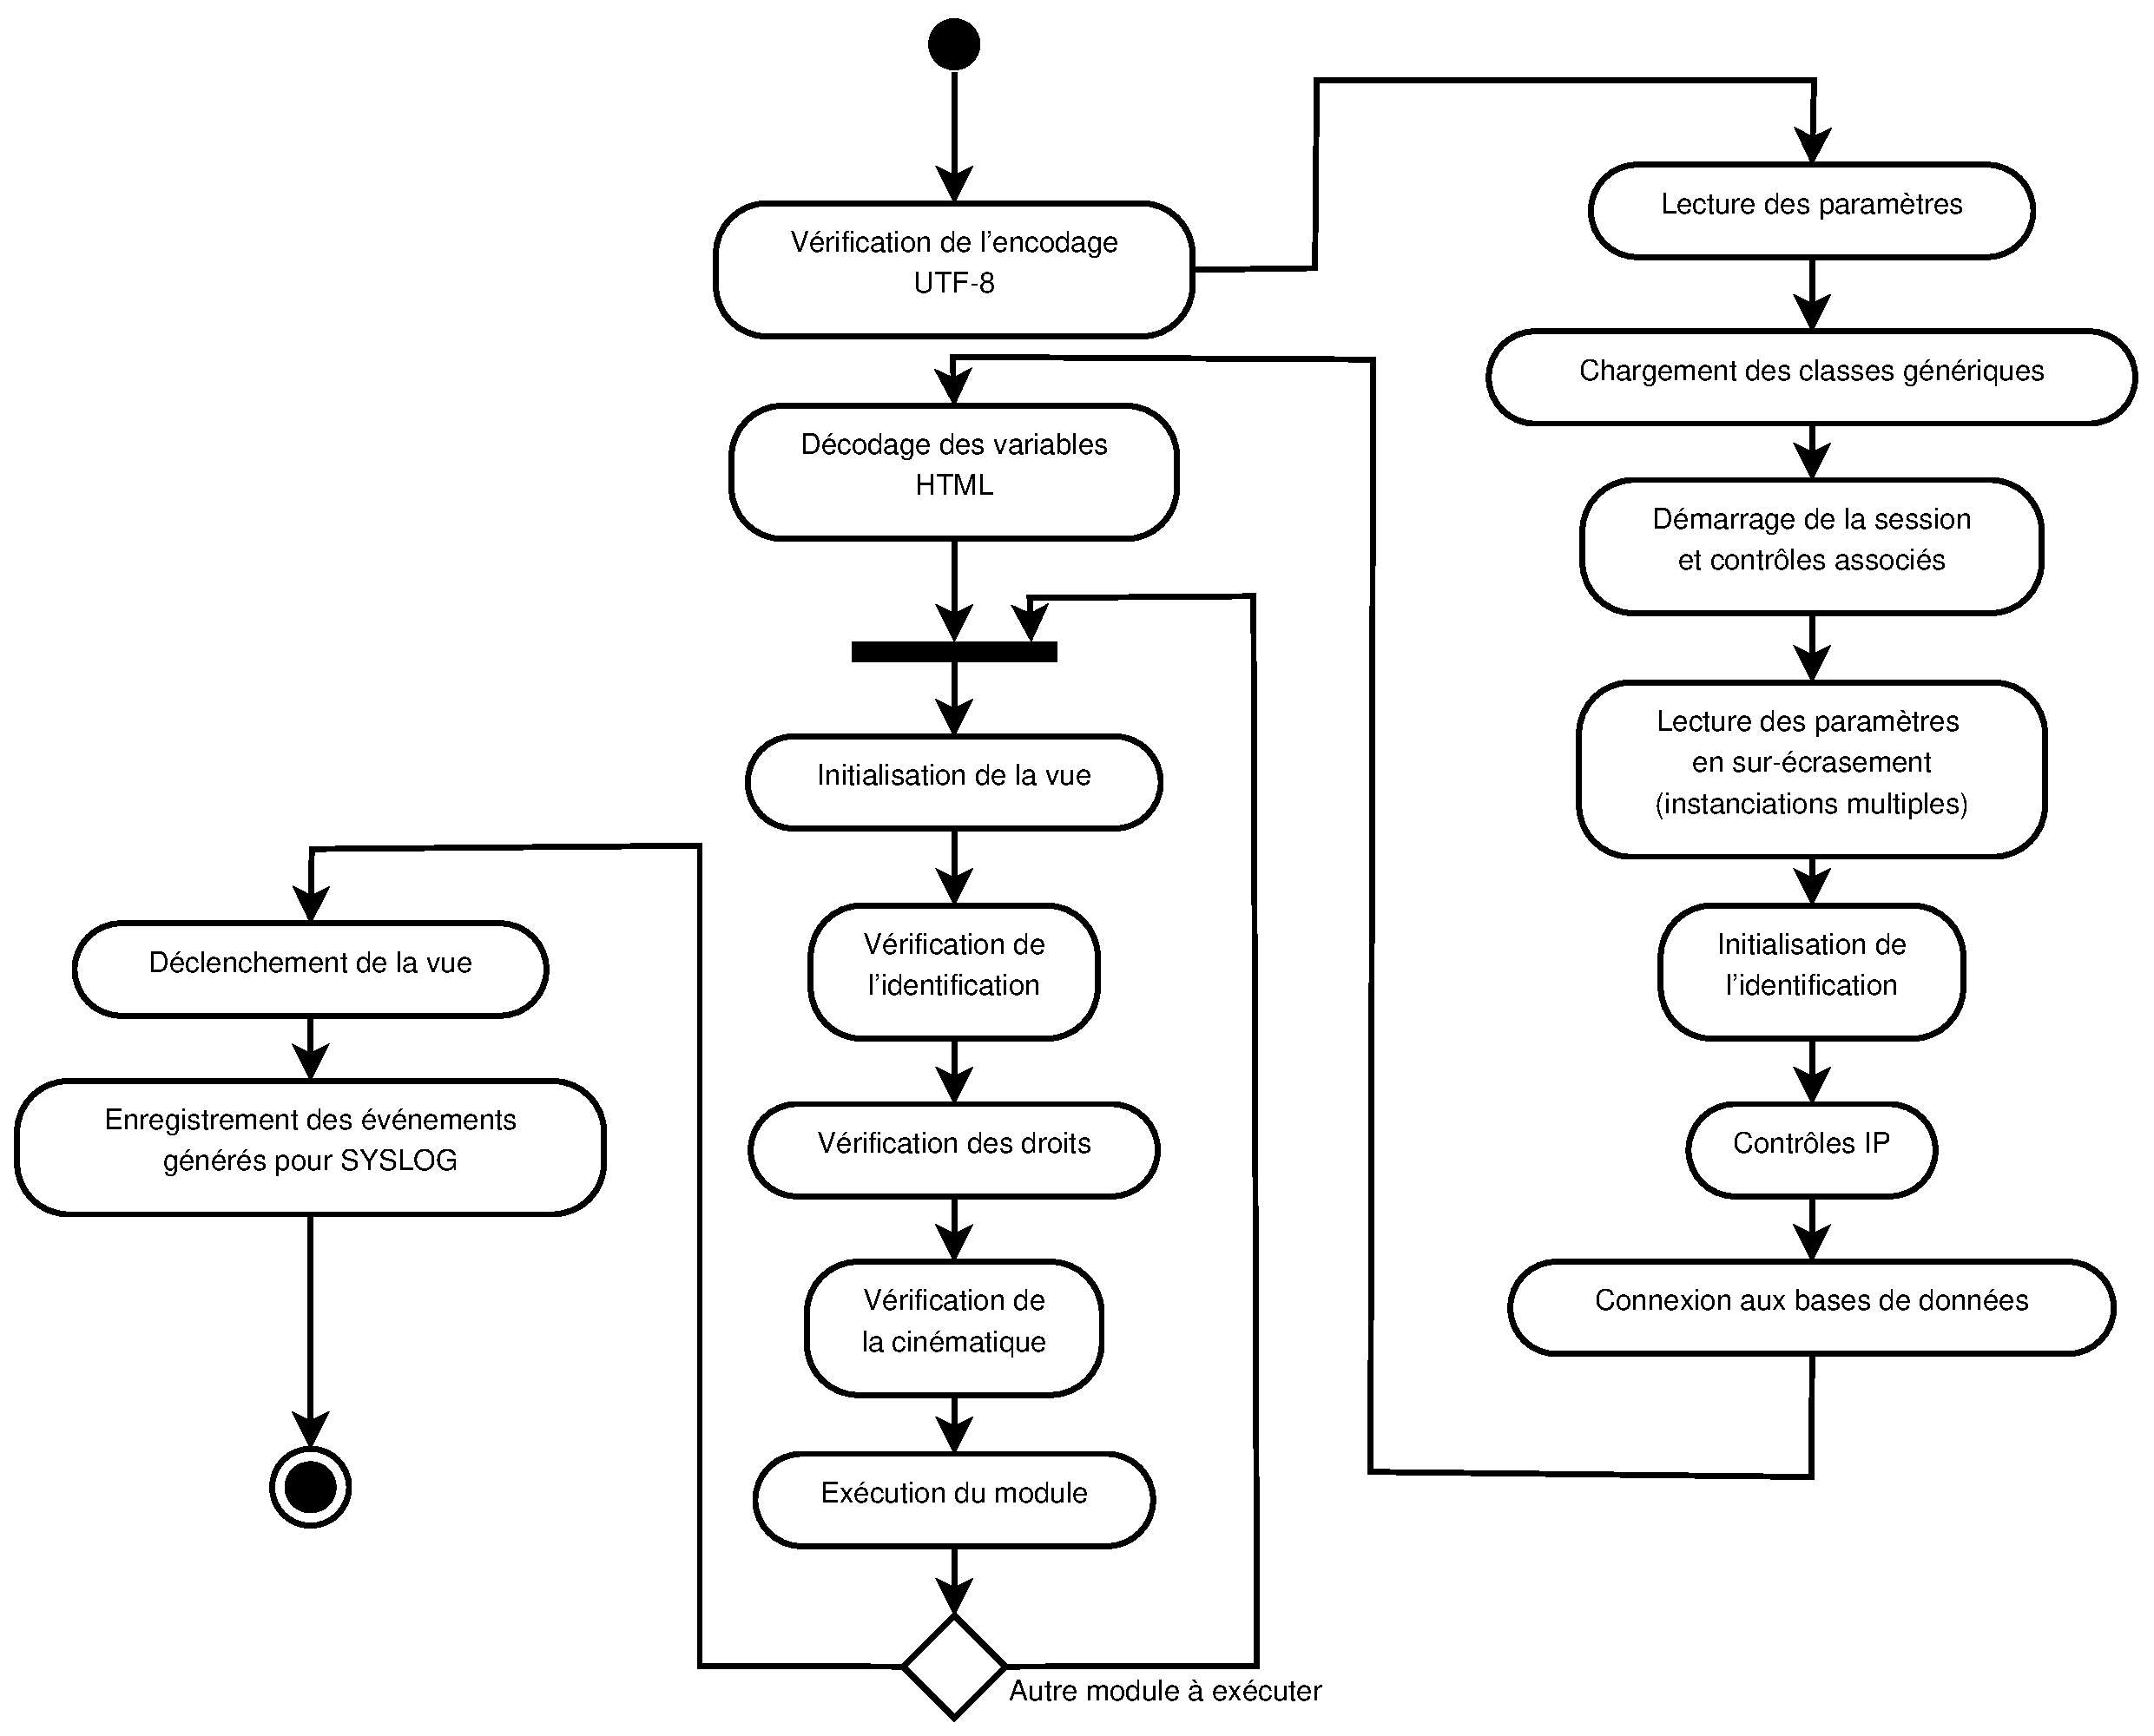
\includegraphics[width=1.2\linewidth]{dessin/synopsis}
\caption{Synopsis général de fonctionnement du contrôleur}
\end{figure}



\section{Synopsis}

L'appel de toute page dans l'application passe nécessairement par l'ensemble de ces étapes :
\begin{itemize}
\item vérification que l'encodage des caractères transmis respecte bien l'encodage utf-8
\item lecture des paramètres
\item chargement des classes génériques utilisées systématiquement
\item démarrage de la session, et ajout de contrôles (durée de la session ouverte...)
\item lecture des paramètres en sur-écrasement, ce qui permet des implémentations multiples avec le même code
\item initialisation de l'identification
\item contrôles de cohérence IP (vérification que, pour une même session, l'adresse IP ne change pas)
\item lancement des connexions aux bases de données (par défaut, deux connexions : une pour la base des droits, l'autre pour les données applicatives)
\item décodage des variables HTML encodées (protection contre les attaques de type XSS)
\item traitement du module demandé :
\begin{itemize}
\item initialisation, le cas échéant, de la vue associée 
\item vérification de l'identification, ou déclenchement des procédures d'identification
\item vérification des droits nécessaires pour accéder au module
\item vérification, le cas échéant, de la cinématique : les opérations de modification ne devraient être possibles que si l'opération précédente correspond à l'affichage du formulaire de saisie
\item exécution du module
\item analyse du code de retour du module, et enchaînement le cas échéant sur un autre module
\end{itemize}
\item déclenchement de la vue 
\item enregistrement, le cas échéant, des messages destinés à SYSLOG (messages systèmes)
\end{itemize}

\section{Organisation des dossiers}
Les fichiers sont organisés selon cette arborescence :
\begin{itemize}
\item \textbf{database} : dossier de travail contenant la description de la base de données, la documentation pour les développeurs, les scripts. Le dossier doit être supprimé lors de la mise en production
\item \textbf{display} : le seul dossier accessible. Il contient tous les fichiers nécessaires pour gérer l'affichage :
\begin{itemize}
\item \textbf{CSS} : les feuilles de style
\item \textbf{images} : les icônes et images utilisées dans l'affichage des pages
\item \textbf{javascript} : l'ensemble des librairies Javascript utilisées
\item \textbf{templates} : les modèles de documents utilisés par Smarty (cf. \ref{smarty}, \textit{\nameref{smarty}}, page \pageref{smarty})
\item \textbf{templates\_c} : dossier utilisé par Smarty pour compiler les templates. Ce dossier doit être accessible en écriture par le serveur Web
\end{itemize}
\item \textbf{doc} : ancien dossier, contenant un mécanisme de gestion de la documentation en ligne. N'est plus utilisé actuellement, mais pourrait être employé le cas échéant
\item \textbf{framework} : le code de base du framework. Il comprend :
\begin{itemize}
\item \textbf{droits} : dossier permettant de gérer les droits 
\item \textbf{identification} : gestion de la connexion des utilisateurs
\item \textbf{import/import.class.php} : classe créée il y a quelques années pour gérer les imports (obsolète en grande partie)
\item \textbf{ldap/ldap.class.php} : connexion à un annuaire LDAP et récupération d'informations
\item \textbf{navigation} : programmes utilisés pour générer le menu et décoder les actions demandées à partir du fichier XML les contenant
\item \textbf{translateId/translateId.class.php} : classe permettant de transcoder les identifiants des enregistrements de la base de données, pour éviter les attaques par forçage de clé
\item de nombreux fichiers utilisés par le framework, dont le contrôleur (controller.php), des fonctions génériques (fonctions.php)...
\item \textbf{vue.class.php} : les classes utilisées pour les vues (cf. \ref{vue} \textit{\nameref{vue}}, page \pageref{vue})
\end{itemize}
\item \textbf{install} : contient des scripts d'installation de la base de données (normalement à déplacer dans \textit{database}), et le fichier \textbf{readme.txt}, décrivant les dernières nouveautés
\item \textbf{locales} : dossier contenant les fichiers de langue (fr.php et en.php)
\item \textbf{modules} : dossier contenant le code spécifique de l'application. Il est organisé ainsi :
\begin{itemize}
\item \textbf{classes} : les classes nécessaires pour l'application
\item \textbf{example} : des exemples de codage
\item les autres dossiers sont libres et contiennent les modules de l'application
\item \textbf{beforeDisplay.php} : fichier appelé systématiquement avant l'affichage des pages HTML
\item \textbf{beforesession.inc.php} : fichier appelé systématiquement avant le démarrage de la session. Il permet de déclarer les librairies qui sont nécessaires pour instancier des classes stockées en variables de session
\item \textbf{common.inc.php} : fichier appelé systématiquement avant le traitement des modules
\item \textbf{fonctions.php} : fonctions déclarées par le programmeur et disponibles dans toute l'application 
\item \textbf{postLogin.php} : script exécuté uniquement quand un utilisateur s'est identifié
\end{itemize}
\item \textbf{param} : dossier contenant les paramètres de l'application :
\begin{itemize}
\item \textbf{actions.xml} : fichier contenant la description de l'ensemble des modules utilisables, avec les droits associés et le type de vue à utiliser
\item \textbf{menu.xml} : description du menu qui sera généré
\item \textbf{param.default.inc.php} : les paramètres par défaut
\item \textbf{param.inc.php} : paramètres en écrasement, spécifiques de l'implémentation. Ce fichier n'est jamais livré lors des mises à jour, pour éviter la suppression des paramètres de base de données, par exemple
\item \textbf{param.inc.php.dist} : fichier d'exemple de \textit{param.inc.php}, à renommer et à mettre à jour lors de l'installation d'une nouvelle implémentation
\end{itemize}
\item \textbf{plugins} : dossier contenant les bibliothèques tierces, comme Smarty, ObjetBDD (maintenant intégré au framework)...
\item \textbf{temp} : dossier de stockage temporaire, qui doit être accessible en écriture au serveur web. Les fichiers présents dans celui-ci ont une durée de vie de 24 heures (suppression lors de la connexion d'un utilisateur)
\item \textbf{test} : dossier utilisé pour réaliser certains tests. Doit être systématiquement supprimé lors de la mise en production
\end{itemize}

Seuls le fichier index.php, à la racine, les dossiers display et test sont accessibles directement. Les autres dossiers sont protégés par des fichiers .htaccess.

\section{Paramètres}

Les paramètres utilisés dans l'application sont gérés avec 3 fichiers différents :
\begin{itemize}
\item \textbf{param/param.default.inc.php} : contient l'ensemble des paramètres utilisés ;
\item \textbf{param/param.inc.php} : contient ceux issus du fichier précédent, qui sont adaptés à l'implémentation ;
\item \textbf{param.ini} : fichier contenant les paramètres spécifiques du nom DNS de l'application (par exemple, schéma particulier associé au nom du site). Pour plus d'informations sur ce point, consultez le chapitre \ref{dnsmultiple} \textit{\nameref{dnsmultiple}}, page \pageref{dnsmultiple}.
\end{itemize}

Voici la description de l'ensemble des paramètres :

\subsection{Paramètres généraux}
% \usepackage{array} is required
\begin{longtable}{|p{5cm}|p{8cm}|}
\hline
\textbf{Variable} & \textbf{Signification} \\
\hline
\endhead
APPLI\_version & Numéro de version de l'application \\ 
\hline 
APPLI\_versiondate & Date de la version \\ 
\hline 
language & Langue par défaut \\
\hline
DEFAULT\_formatdate & Format par défaut d'affichage des dates\\
\hline
navigationxml & nom du fichier XML contenant la description des modules exécutables\\
\hline
APPLI\_session\_ttl & durée de la session, en secondes\\
\hline
APPLI\_cookie\_ttl & durée de vie par défaut des cookies, en secondes\\
\hline
APPLI\_path\_stockage\_session & obsolète\\
\hline
LOG\_duree & Durée de conservation des traces des actions réalisées, en jours\\
\hline
APPLI\_mail & Adresse pour déclarer les incidents (mail ou non)\\
\hline
APPLI\_titre & Nom de l'application qui sera affiché (cas où le code est utilisé par plusieurs entrées différentes) \\
\hline
APPLI\_code & Code interne de l'application. Utilisé dans certains cas\\
\hline
APPLI\_fds & Feuille de style utilisée par défaut (obsolète)\\
\hline
APPLI\_address & Adresse DNS de l'application. Utilisée en cas d'identification CAS (adresse de retour)\\
\hline
APPLI\_modeDeveloppement & si à true, certaines opérations sont réalisées dans un contexte de développement (affichage de messages, recalcul systématique du menu...)\\
\hline
APPLI\_notSSL & utilisé en développement, si l'application ne fonctionne pas en mode SSL (déconseillé) \\
\hline
APPLI\_utf8 & systématiquement à true (plus de support des autres encodages)\\
\hline
APPLI\_menufile & nom du fichier XML contenant la description du menu\\
\hline
APPLI\_temp & nom du dossier utilisé pour stocker les fichiers temporaires\\
\hline
APPLI\_moduleDroitKO & nom du module appelé en cas de refus d'accès pour un problème de droits \\
\hline
APPLI\_moduleErrorBefore & nom du module appelé en cas de problème lié à la cinématique de l'application\\
\hline
APPLI\_moduleNoLogin & nom du module appelé en cas d'échec d'identification \\
\hline
paramIniFile & nom du fichier contenant les paramètres spécifiques liés au DNS utilisé (\textit{cf.} \ref{dnsmultiple} \textit{\nameref{dnsmultiple}}, page \pageref{dnsmultiple}) \\
\hline
SMARTY\_param & Paramètres utilisés par le moteur de templates SMARTY\\
\hline
SMARTY\_variables & variables systématiquement transmises à SMARTY et utilisées lors de l'affichage général\\
\hline
ERROR\_display & Affiche les erreurs à l'écran (mode développement)\\
\hline
OBJETBDD\_debugmode & 0 : pas d'affichage de message d'erreur, 1, affichage des messages d'erreur, 2 : affichage de toutes les commandes SQL générées par ObjetBDD \\
\hline
ADODB\_debugmode & obsolète \\
\hline
\caption{Variables générales de l'application}
\end{longtable} 

\subsection{Identification}
\begin{longtable}{|p{5cm}|p{8cm}|}
\hline
\textbf{Variable} & \textbf{Signification} \\
\hline
\endhead
ident\_type & Type d'identification supporté. L'application peut gérer \textbf{BDD} (uniquement en base de données),\textbf{LDAP} (uniquement à partir d'un annuaire LDAP) \textbf{LDAP-BDD} (d'abord identification en annuaire LDAP, puis en base de données), et \textbf{CAS} (serveur d'identification \textit{Common Access Service})\\
\hline
CAS\_plugin & Nom du plugin utilisé pour une connexion CAS \\
\hline
CAS\_address & Adresse du serveur CAS\\
\hline
CAS\_port & Systématiquement 443 (connexion chiffrée)\\
\hline
LDAP & tableau contenant tous les paramètres nécessaires pour une identification LDAP \\
\hline
privateKey & clé privée utilisée pour générer les jetons d'identification \\
\hline
pubKey & clé publique utilisée pour générer les jetons d'identification \\
\hline
tokenIdentityValidity & durée de validité, en secondes, des jetons d'identification\\
\hline
\caption{Variables utilisées pour paramétrer l'identification}
\end{longtable}

Voici le contenu des variables du tableau LDAP : 
\begin{longtable}{|p{5cm}|p{8cm}|}
\hline
\textbf{Variable} & \textbf{Signification} \\
\hline
\endhead
address &  adresse de l'annuaire\\
\hline
port & 389 en mode non chiffré, 636 en mode chiffré\\
\hline
rdn & compte de connexion, si nécessaire \\
\hline
basedn & base de recherche des utilisateurs\\
\hline
user\_attrib & nom du champ contenant le login à tester\\
\hline
v3 & toujours à \textit{true}\\
\hline
tls & \textit{true} en mode chiffré\\
\hline
groupSupport & \textbf{true} si l'application recherche les groupes d'appartenance du login dans l'annuaire\\
\hline
groupAttrib & Nom de l'attribut contenant la liste des groupes d'appartenance\\
\hline
commonNameAttrib & Nom de l'attribut contenant le nom de l'utilisateur\\
\hline
mailAttrib & Nom de l'attribut contenant l'adresse mail de l'utilisateur\\
\hline
attributgroupname & Attribut contenant le nom du groupe lors de la recherche des groupes (cn par défaut)\\
\hline
attributloginname & attribut contenant les membres d'un groupe\\
\hline
basedngroup & base de recherche des groupes \\
\hline
\caption{Variables utilisées pour paramétrer l'accès à l'annuaire LDAP}
\end{longtable}

\subsection{Connexions aux bases de données}

Deux connexions sont systématiquement implémentées : l'une à la base de données contenant la gestion des droits, et l'autre à celle contenant les données propres à l'application.
\begin{longtable}{|p{5cm}|p{8cm}|}
\hline
\textbf{Variable} & \textbf{Signification} \\
\hline
\endhead
BDD\_login & compte de connexion à la base de données \\
\hline
BDD\_passwd & mot de passe associé\\
\hline
BDD\_dsn & adresse de la base de données sous forme normalisée\\
\hline
BDD\_schema & schéma utilisé (plusieurs schémas peuvent être décrits, en les séparant par une virgule - fonctionnement propre à Postgresql)\\
\hline
GACL\_dblogin & compte de connexion à la base de données des droits\\
\hline
GACL\_dbpasswd & mot de passe associé\\
\hline
GACL\_dsn & adresse normalisée \\
\hline
GACL\_schema & schéma utilisé\\
\hline
GACL\_aco & nom du code de l'application utilisé dans la gestion des droits (\textit{cf.} \ref{droits} \textit{\nameref{droits}}, page \pageref{droits} )\\
\hline


\caption{Variables utilisées pour paramétrer les connexions}
\end{longtable}

Il est possible de créer des comptes séparés, voire de ne donner accès qu'en lecture à la base des droits (à l'exception de la table \textit{log}, qui contient la trace de toutes les actions demandées).

\chapter{Décrire les actions}

Les actions possibles dans le logiciel sont décrites dans un fichier, par défaut \textit{param/actions.xml}. C'est un fichier XML dont la racine s'appelle \textit{navigation}. 

Une action est la conjonction entre un contexte et une opération, par exemple \textit{poissonList} pour afficher la liste des poissons, \textit{poissonChange} pour afficher la page de modification d'un poisson, \textit{poissonWrite} ou \textit{poissonDelete} pour déclencher l'écriture en base de données.

Dans le contexte de ce framework, l'action s'appelle \textit{module} (nom du champ transmis depuis le navigateur). L'attribut \textit{action} contient le nom du fichier PHP appelé. Il est associé à l'attribut \textit{param}, qui permet d'indiquer le détail de l'action à réaliser (par exemple, \textit{list} ou \textit{change}).

Voici la liste des attributs disponibles pour un module (ou une action) :
\begin{longtable}{|p{2.5cm}|c|p{9cm}|}
\hline
\textbf{Attribut} & \textbf{Requis} & \textbf{Signification} \\
\hline
\endhead
action & X & nom de la page PHP à exécuter (accès relatif depuis la racine de l'application) \\
 \hline
param &  & paramètre analysé dans la page, pour savoir quelle action doit être réalisée. Par convention, les actions possibles sont les suivantes : list, read, change, write, delete, ou autre action \\
 \hline
droits &  & Liste des droits nécessaires pour exécuter l'action. Si plusieurs droits sont possibles, ils doivent être séparés par une virgule\\
 \hline
loginrequis & & Indique, en l'absence de droits spécifiques, si l'action nécessite d'être connecté. Vaut 1 si la connexion est requise\\
 \hline
modulebefore & & Pour les opérations d'écriture, permet d'indiquer le nom du module qui doit impérativement être exécuté avant. Cela limite les risques d'attaques de type CSRF et les rafraîchissements intempestifs dans les formulaires. Plusieurs modules peuvent être indiqués, en les séparant par une virgule\\
 \hline
retourok & & indique le nom du module qui sera exécuté si le code de retour (variable \$module\_coderetour) vaut 1 \\
 \hline
retourko & & indique le nom du module qui sera exécuté si le code de retour (variable \$module\_coderetour) vaut -1 (échec d'exécution) \\
 \hline
type & (X) & pour les modules envoyant des données au navigateur, indique le type de la vue qui sera utilisée. Les valeurs possibles sont smarty ou html (même vue), ajax, pdf, csv  \\
 \hline
droitko & & nom du module appelé si les droits ne sont pas suffisants pour exécuter l'action demandée \\
\hline 
 
 \caption{Liste des attributs utilisables pour décrire une action}\label{actions}
\end{longtable}

Le module \textit{model} n'est pas analysé, il sert à montrer l'ensemble des options possibles. 

Le module \textit{default} correspond au module appelé par défaut, si l'application est appelée sans indiquer de nom de module (variable \textit{module} non transmise soit dans le lien, soit dans le formulaire).

Voici quelques exemples d'utilisation :
\begin{lstlisting}
	<appliList action="framework/droits/appli.php" param="list" droits="admin" retourlogin="1"  type="smarty" />
	<appliDisplay action="framework/droits/appli.php" param="display" droits="admin"  type="smarty"/>
	<appliChange action="framework/droits/appli.php" param="change" droits="admin"  type="smarty"/>
	<appliWrite action="framework/droits/appli.php" param="write" droits="admin" retourok="appliDisplay" retourko="appliChange" modulebefore="appliChange" />
	<appliDelete action="framework/droits/appli.php" param="delete" droits="admin" retourok="appliList" retourko="appliChange"  modulebefore="appliChange"/>
\end{lstlisting}

Il s'agit des modules utilisés dans la gestion des droits. Ils nécessitent tous que l'utilisateur dispose du droit \textit{admin}. Une seule page est appelée (\textit{appli.php}), l'action à réaliser étant analysée à partir de l'attribut \textit{param}.

Les modules \textit{appliWrite} et \textit{appliDelete} ne génèrent pas directement d'affichage : ils sont là uniquement pour écrire des informations dans la base de données. Par contre, ils enchaînent, en fonction de leur code de retour, soit sur le réaffichage du formulaire de saisie, soit sur le retour au détail ou à la liste.
Ces deux modules ne peuvent être exécutés que si le précédent est \textit{appliChange}, c'est à dire si le formulaire de saisie a été affiché.

\chapter{Identifier les utilisateurs et gérer les droits}\label{droits}
\part{Le modèle}
\chapter{ObjetBDD - accéder aux bases de données}\label{objetbdd}

\section{Présentation}

ObjetBDD est une classe qui sert d'interface entre l'application et la base de données. Elle a été créée pour simplifier les requêtes, seules celles d'interrogation spécifiques devront être écrites.

Historiquement, ObjetBDD travaillait avec ADODB, une classe qui encapsulait la connexion à la base de données. Avec la sortie de PDO, la classe a été adaptée pour utiliser des connexions PDO.
Elle était également prévue pour fonctionner initialement avec Sybase ASE et MySQL. Les récentes évolutions ont porté sur le support des bases PostgreSQL : il n'est pas certain que toutes les fonctionnalités soient disponibles pour MySQL ou Sybase ASE.

Les fonctions initiales ont été modifiées ou complétées pour supporter maintenant les requêtes préparées.

\section{Fonctionnalités générales}
\subsection{Formatage des dates}
Les dates stockées dans les bases de données sont dans un format difficilement utilisable. La classe transforme automatiquement les dates dans le format français par défaut (mais d'autres formats possibles). 

Elle est également capable de transformer les dates reçues du navigateur au format de stockage. Le format de saisie est libre : la plupart des séparateurs sont supportés, l'année est rajoutée automatiquement, etc.

Le formatage des date inclut également les dates/heures.

\subsection{Opérations d'écriture en base de données}

La classe dispose de deux fonctions pour écrire les informations : ecrire() et supprimer(). La fonction ecrire() va décider s'il faut réaliser un insert ou un update, en fonction de la clé fournie. Par convention, si la clé vaut 0, un insert sera réalisé.

\subsection{Gestion des erreurs}

En cas d'échec d'exécution d'une requête SQL, la classe génère une exception.

\section{Variables générales utilisables}

Ces variables sont toutes publiques.
\begin{longtable}{|p{3cm}|c|p{8.5cm}|}
\hline
\textbf{Variable} & \textbf{Type} & \textbf{Signification} \\
\hline
\endhead
connection & PDO & instance PDO. Peut être utilisée pour instancier une nouvelle classe basée sur ObjetBDD à l'intérieur d'une fonction \\
\hline
id\_auto & entier & Si à 1, la classe gère la création automatique des identifiants. Si à 2, l'identifiant est généré manuellement, avec une requête de type \textit{max(id)} \\
\hline
formatDate & entier & 0 : amj, 1 : jma (défaut), 2 : mja \\
\hline
debug\_mode & entier & 0 : pas de mode de débogage, 1 : affichage des messages d'erreur, 2 : affichage de toutes les commandes SQL générées
\\
\hline
error\_data & tableau & liste de toutes les erreurs détectées lors de la vérification des données.  \\
 & & \$errorData[]["code"] : code d'erreur : \\
	& & 0 : non précisé \\
	& & 1 : champ non numérique \\
	& & 2 : champ texte trop grand \\
	& & 3 : masque (pattern) non conforme \\
	& & 4 : champ obligatoire vide \\
	& & \$errorData[]["colonne"] : champ concerne \\
	& & \$errorData[]["valeur"] : valeur initiale \\
\hline
srid & numérique & Valeur du srid pour les variables de type Postgis \\
\hline
quoteIdentifier & caractère & caractère utilisé pour encadrer les noms des colonnes dans les requêtes (pour les colonnes contenant une majuscule ou un accent) \\
\hline
transformComma & entier & Si à 1 (défaut), les virgules sont transformées en points pour les nombres décimaux \\
\hline

\caption{Liste des variables utilisables dans ObjetBDD}

\end{longtable}

En principe, les variables sont initialisées lors de l'instanciation de la classe, mais peuvent être modifiées à la volée, si nécessaire.

La classe est conçue pour fonctionner en UTF8.

\section{Héritage}

La classe ObjetBDD n'est pas instanciable, et doit donc être héritée. En particulier, le constructeur de la classe doit être surchargé pour rendre la classe opérante. 

\section{Fonctions principales}
\subsection{Constructeur de la classe}

\begin{lstlisting}
function __construct(PDO &$p_connection, array $param = array())
\end{lstlisting}
\subsubsection{Paramètres}
La fonction doit recevoir une instance PDO, correspondant à une connexion déjà réalisée à la base de données. Cette instance PDO est stockée ensuite dans la variable \textit{connection}, qui peut être réutilisée si d'autres classes héritées sont à instancier à l'intérieur du code.

Le tableau \textit{param} comprend, si nécessaire, l'ensemble des variables globales à mettre à jour.

\subsubsection{Surcharge}

Le constructeur doit être impérativement être surchargé, avec le code minimal suivant (exemple) : 

\begin{lstlisting}
function __construct($bdd, $param = array()) {
		$this->table = "acllogin";
		$this->colonnes = array (
				"acllogin_id" => array (
						"type" => 1,
						"key" => 1,
						"requis" => 1,
						"defaultValue" => 0 
				),
				"login" => array (
						"requis" => 1 
				),
				"logindetail" => array (
						"type" => 0,
						"requis" => 1 
				) 
		);
		parent::__construct ( $bdd, $param );
	}
\end{lstlisting}

\textit{table} doit correspondre au nom de la table (sans tenir compte du schéma, traité lors de la connexion à la base de données).

\textit{colonnes} contient la description des colonnes de la table. Chaque colonne doit être nommée, et contient un tableau, dont les  attributs possibles sont les suivants :

\begin{longtable}{|p{3cm}|p{10cm}|}
\hline
\textbf{Variable} & \textbf{Signification} \\
\hline
\endhead
type & 0 : varchar \\
& 1 : numérique (y compris décimaux) \\
& 2 : date \\
& 3 : datetime \\
& 4 : champ Postgis \\
\hline
requis & Si à 1, le contenu doit être fourni pour réaliser l'écriture \\
\hline
key & Si à 1, l'attribut est utilisé comme clé primaire (en principe, n'utiliser que des clés mono-attributs, même si la classe devrait être capable de gérer des clés multiples) \\
\hline
defaultValue & valeur par défaut. Il est possible d'indiquer le nom d'une fonction (entre guillemets). Parmi celles-ci, il est possible d'utiliser :\\
& getDateJour : retourne la date du jour \\
& getDateHeure : retourne la date et l'heure courante \\
& getLogin : retourne la valeur de la variable \$\_SESSION["login"]\\
\hline
parentAttrib & si vaut 1, la valeur est utilisée comme clé étrangère principale de l'enregistrement \\
\hline
longueur & pour les champs de type varchar, indique la longueur maximale autorisée (attention au codage UTF-8, les caractères accentués étant comptés pour 2) \\
\hline
pattern & pattern traité par expression régulière, pour tester la correspondance de l'information fournie au modèle décrit \\
\hline

\caption{Liste des attributs permettant de décrire les colonnes de la table\label{objetbdd-attr}}

\end{longtable}

Les deux derniers attributs sont toujours utilisables, mais en rarement employés.

\subsection{lire}
\begin{lstlisting}
lire($id, $getDefault = true, $parentValue = 0)
\end{lstlisting}

Fonction permettant de récupérer un enregistrement. Elle accepte les paramètres suivants :
\begin{longtable}{|p{3cm}|p{10cm}|}
\hline
\textbf{Variable} & \textbf{Signification} \\
\hline
\endhead
id & clé de l'enregistrement \\
\hline
getDefault & si à \textit{true}, récupère les valeurs par défaut si l'enregistrement n'existe pas dans la base (initialisation d'une saisie, par exemple)\\
\hline
parentValue & clé de l'enregistrement parent. Si \textit{getDefault} vaut \textit{true}, pré-remplit l'attribut qui contient la valeur \textit{parentAttrib} avec la clé fournie dans \textit{parentValue} \\
\hline

\caption{Liste des paramètres de la fonction lire}
\end{longtable}

La fonction retourne le tableau associatif correspondant.

\subsection{ecrire}
\begin{lstlisting}
ecrire($data)
\end{lstlisting}
Déclenche l'écriture des informations dans la base de données. \$data doit être un tableau qui comprend les attributs à écrire (au minimum, les attributs déclarés comme obligatoires).

Le nom des attributs fournis doit correspondre exactement au nom des colonnes.

En principe, ce tableau correspond à la variable \$\_REQUEST.

La fonction génère soit une commande insert, soit une commande update. En principe, la commande insert est générée si la clé fournie vaut 0.

Elle retourne la clé modifiée ou créée.

\subsection{supprimer}

\begin{lstlisting}
supprimer($id)
\end{lstlisting}

Permet de supprimer un enregistrement, à partir de sa clé. Attention : la fonction ne gère pas les suppressions en cascade, si ce n'est pas prévu directement dans la base de données.

\subsection{supprimerChamp}

\begin{lstlisting}
supprimerChamp($id, $champ)
\end{lstlisting}

Fonction très pratique pour supprimer tous les enregistrements fils. Elle génère une requête du type :
\begin{lstlisting}
delete from table where :champ = :id;
\end{lstlisting}


\subsection{getListe}

\begin{lstlisting}
getListe($order = "")
\end{lstlisting}

Fonction récupérant l'ensemble des enregistrements d'une table, triés ou non selon le contenu de la variable \$order.

\subsection{getListFromParent}

\begin{lstlisting}
function getListFromParent($parentId, $order = "")
\end{lstlisting}

Retourne la liste des enregistrements fils correspondant à la clé étrangère \$parentId. Le résultat peut ou non être trié selon les paramètres définis dans la seconde variable.

\subsection{getListParamAsPrepared}

\begin{lstlisting}
function getListeParamAsPrepared($sql, $data)
\end{lstlisting}

Permet de récupérer une liste d'enregistrements à partir de la requête SQL fournie et du tableau des données à insérer (requêtes préparées PDO), avec transformation des dates

\subsection{getListeParam}
\begin{lstlisting}
function getListeParam($sql)
\end{lstlisting}

Exécute la requête et retourne la liste des enregistrements correspondants, avec transformation des dates.

Attention : cette fonction ne gère pas la préparation des requêtes : il importe au codeur d'en tenir compte pour éviter les risques d'injection de code. Elle ne devrait être utilisée que dans les cas où une requête préparée ne peut être utilisée.

\subsection{ecrireTableNN}

\begin{lstlisting}
ecrireTableNN($nomTable, $nomCle1, $nomCle2, $id, $lignes)
\end{lstlisting}

Fonction permettant de mettre à jour les tables de relation NN, selon le schéma suivant :

\begin{figure}[H]
\centering
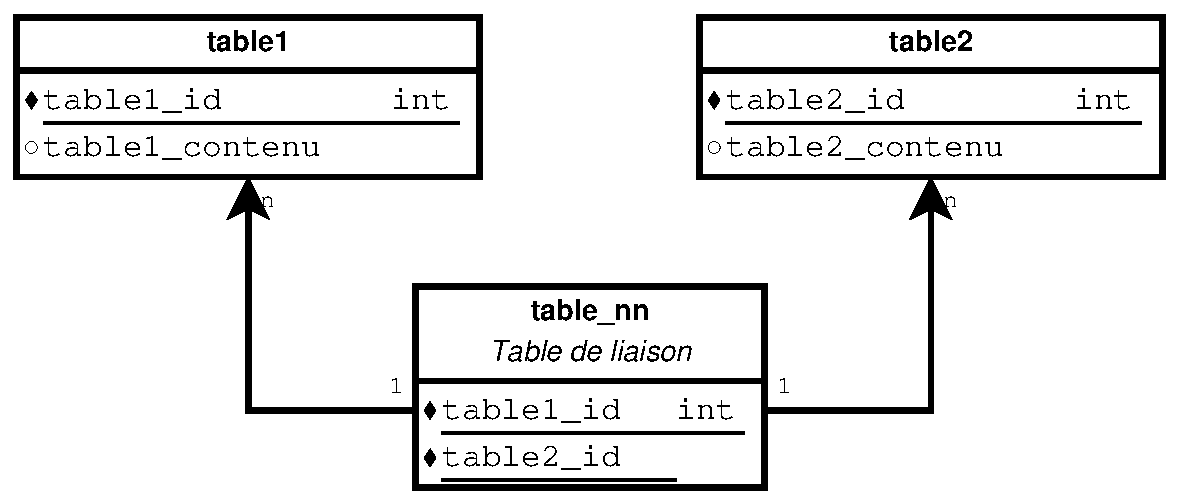
\includegraphics[width=0.8\linewidth]{dessin/schema-nn}
\caption{Structure d'une liaison N-N}
\end{figure}

En général, la saisie de ce type de liaisons est effectuée par des cases à cocher, ce qui permet de récupérer un tableau contenant la liste des clés de la table2 (champs html \textit{<input type checkbox name="attribut[]">}).

Les arguments à indiquer sont les suivants :
\begin{longtable}{|p{3cm}|p{10cm}|}
\hline
\textbf{Variable} & \textbf{Signification} \\
\hline
\endhead
nomTable & Nom de la table NN (table\_nn dans notre exemple) \\
\hline
nomCle1 & nom de l'attribut contenant la clé de la table principale \\
\hline
nomCle2 & nom de l'attribut contenant les clés de la table secondaire \\
\hline
id & valeur de la clé de la table principale \\
\hline
lignes & tableau contenant les valeurs de la table secondaire à conserver ou à rajouter \\
\hline

\caption{Liste des paramètres de la fonction ecrireTableNN}
\end{longtable}

La fonction ne génère que les requêtes de modification nécessaires (insertion ou suppression). Elle permet d'éviter de déclarer une instanciation d'ObjetBDD pour la table\_nn.

\subsection{getBlobReference}

\begin{lstlisting}
function getBlobReference($id, $fieldName)
\end{lstlisting}

Fonction permettant de récupérer un champ binaire stocké dans la base de données. PDO retourne l'identifiant interne PHP du fichier temporaire contenant l'information binaire lu.

Arguments :
\begin{longtable}{|p{3cm}|p{10cm}|}
\hline
\textbf{Variable} & \textbf{Signification} \\
\hline
\endhead
id & Clé de l'enregistrement \\
\hline
fieldName & nom de la colonne contenant l'information binaire \\
\hline
\caption{Liste des paramètres de la fonction getBlobReference}
\end{longtable}

\subsection{encodeData}

\begin{lstlisting}
encodeData($data)
\end{lstlisting}

Fonction encodant les quottes comprises dans les champs du tableau data, pour toutes les requêtes SQL directes (exécution ne passant pas par le mécanisme des requêtes préparées).

\subsection{executeAsPrepared}

\begin{lstlisting}
function executeAsPrepared($sql, $data, $onlyExecute = false) 
\end{lstlisting}

Fonction exécutant la requête fournie sous forme de requête préparée. Les variables à insérer sont décrites dans le tableau \textit{data}. Si l'attribut \$onlyExecute vaut true, la fonction ne retourne pas de résultat.

\subsection{executeSQL}

\begin{lstlisting}
function executeSQL($ls_sql) {
\end{lstlisting}

Exécute la commande SQL, sans précaution particulière (attention aux risques d'injection).

\subsection{formatDateDBversLocal}

\begin{lstlisting}
function formatDateDBversLocal($date, $type = 2)
\end{lstlisting}

Transforme la date, au format de la base de données, vers le format lisible pour l'utilisateur.

Si \$type vaut 3, la fonction retourne le champ au format date/heure.

\subsection{formatDateLocaleVersDB}
\begin{lstlisting}
function formatDateLocaleVersDB($date, $type = 2)
\end{lstlisting}

Transforme la date fournie en format géré par la base de données. Si le type vaut 3, un champ de type date/heure est attendu.

\subsection{utilDatesDBVersLocale}
\begin{lstlisting}
function utilDatesDBVersLocale($data)
\end{lstlisting}

Transforme les dates présentes dans le tableau joint à un format lisible par l'utilisateur.

\begin{lstlisting}
function utilDatesLocaleVersDB($data)
\end{lstlisting}

Transforme les dates présentes dans le tableau joint au format supporté par la base de données.

\section{Utilisation avancée}
\subsection{Requête multi-table contenant des champs date}
Un des cas fréquents posé par ObjetBDD est celui des requêtes manuelles qui retournent des dates. L'objectif est de les formater pour les mettre dans le même état que les dates décrites dans la table associée à la classe.

Le plus simple consiste à rajouter la colonne date complémentaire à la liste des variables juste avant d'exécuter la requête. Voici un exemple :
\begin{lstlisting}
$sql = "select t1.id, t1.date1, t2.id2, t2.date2
from table1 t1
join table2 t2 using (id)";
$this->colonnes["date2"]=array("type"=>2);
return $this->getListeParam($sql);
\end{lstlisting}

Une fois le contenu de la requête récupéré, la classe pourra alors appliquer la transformation de date sur la colonne issue de la  seconde table.

\section{Le tableau de paramètres ObjetBDDParam}\label{objetbddparam}

ObjetBDDParam est une variable contenant les paramètres par défaut utilisés pour initialiser les instances issues d'ObjetBDD. C'est en particulier assez pratique pour gérer le choix de la langue d'affichage pour les dates. Il est également possible de modifier, de manière globale dans le logiciel, le fonctionnement d'ObjetBDD.

Ce tableau devrait être passé systématiquement en paramètre de toute instanciation d'objet basé sur ObjetBDD.

\chapter{Exécuter les actions}
Le framework est conçu pour n'exécuter que les actions décrites dans un fichier XML (\textit{cf.} \ref{labelxml} \textit{\nameref{labelxml}}, page \pageref{labelxml}).

Les actions sont identifiées par deux informations : d'une part, le nom du fichier PHP à exécuter, et d'autre part un paramètre permettant de décrire ce qu'il faut réaliser précisément. Ce second paramètre pourrait ne pas être utilisé, mais cela impliquerait un fichier par action. 
Le framework a été conçu pour obtenir un bon équilibre entre le nombre de fichiers et la navigation dans le code.

\section{Les actions standard}

En général, on identifie facilement les actions suivants sur un type d'objet :
\begin{itemize}
\item l'affichage d'une boite de recherche et de la liste des dossiers correspondants ;
\item l'affichage du détail d'un enregistrement ;
\item l'affichage de la page permettant de créer ou de modifier un enregistrement ;
\item l'écriture des informations en base de données ;
\item la suppression d'une fiche.
\end{itemize}

Par convention, ces actions sont nommées \textbf{list}, \textbf{display}, \textbf{change}, \textbf{write} et \textbf{delete}. 

Voici un exemple de code standard utilisé pour traiter tous les modules (fichier modules/example/example.php, à recopier et à adapter...) :

\begin{lstlisting}
include_once 'modules/example/example.class.php';
$dataClass = new Example($bdd,$ObjetBDDParam);
$keyName = "example_id";
$id = $_REQUEST[$keyName];

switch ($t_module["param"]) {
	case "list":
		/*
		 * Display the list of all records of the table
		 */
		 /*
		 * $searchExample must be defined into modules/beforesession.inc.php :
		 * include_once 'modules/classes/searchParam.class.php';
		 * and into modules/common.inc.php :
		 * if (!isset($_SESSION["searchExample"])) {
    	 * $searchExample = new SearchExample();
		 *	$_SESSION["searchExample"] = $searchExample; 
		 *	} else {
		 *	$searchExample = $_SESSION["searchExample"];
		 *	}
		 * and, also, into modules/classes/searchParam.class.php...
		 */
		 $searchExample->setParam ( $_REQUEST );
		 $dataSearch = $searchExample->getParam ();
		if ($searchExample->isSearch () == 1) {
			$data = $dataClass->getListeSearch ( $dataExample );		
		$vue->set($data , "data");
		$vue->set(1, "isSearch");
		}
		$vue->set($dataSearch, "exampleSearch");
		$vue->set("example/exampleList.tpl","corps" );
		break;
	case "display":
		/*
		 * Display the detail of the record
		 */
		$data = $dataClass->lire($id);
		$vue->set($data,"data");
		/*
		 * Assignation du modele d'affichage
		 */
		$vue->set(  "example/exampleDisplay.tpl", "corps");

		break;
	case "change":
		/*
		 * open the form to modify the record
		 * If is a new record, generate a new record with default value :
		 * $_REQUEST["idParent"] contains the identifiant of the parent record 
		 */
		dataRead($dataClass, $id, "example/exampleChange.tpl", $_REQUEST["idParent"]);
		break;
	case "write":
		/*
		 * write record in database
		 */
		$id = dataWrite($dataClass, $_REQUEST);
		if ($id > 0) {
			$_REQUEST[$keyName] = $id;
		}
		break;
	case "delete":
		/*
		 * delete record
		 */
		dataDelete($dataClass, $id);
		break;
}
\end{lstlisting}

Quelques explications...

Le code commence par charger la classe héritée d'ObjetBDD, puis celle-ci est instanciée avec, en paramètres, la connexion PDO à utiliser et le tableau \textit{ObjetBDDParam}, qui contient la configuration par défaut d'ObjetBDD (\textit{cf.} \ref{objetbddparam} \textit{\nameref{objetbddparam}}, page \pageref{objetbddparam}).

Le nom de la clé associée est indiqué, ce qui permet d'obtenir une code plus générique.

Ensuite, le tableau contenant la description de l'action (t\_param) est analysé, et plus particulièrement sa valeur \textit{param}, qui correspond à ce qu'on attend du module, avec une instruction \textit{switch}.

Quelques précisions sur ce qui est implémenté par défaut.

\subsection{list}

Permet d'afficher une boite de recherche et la liste des dossiers associés. 

\subsubsection{La classe de gestion des critères de recherche}

Les paramètres de recherche peuvent être stockés en variable de session, pour que l'utilisateur récupère la liste des dossiers affichés précédemment quand il revient sur cet écran. 

Chaque jeu de paramètres est déclaré dans une instance héritée de la classe \textit{SearchParam}, dans le fichier \textit{modules/classes/search.class.php}.

Voici un exemple d'instanciation de cette classe de recherche :
\begin{lstlisting}
class SearchExample extends SearchParam {
	function __construct() {
		$this->param = array (
				"comment" => "",
				"numero" => 0,
				"numero1" => "",
				"dateExample" => date ( 'd/m/Y' ) 
		);
		$this->paramNum = array (
				"numero",
				"numero1" 
		);
		parent::__construct ();
	}
}
\end{lstlisting}

Deux tableaux doivent être déclarés. Le premier correspond aux attributs utilisables dans la recherche, et leur valeur par défaut doit être indiquée. Le second indique quels sont les champs qui sont numériques.

Deux fonctions sont utilisés couramment : 
\begin{itemize}
\item setParam(\$\_REQUEST) : met à jour les paramètres de recherche ;
\item getParam() : retourne le tableau avec les paramètres de recherche.
\end{itemize}

De plus, une fonction utilitaire permet de savoir s'il s'agit de la première fois que la recherche est utilisée. Si le formulaire contient un champ configuré ainsi :
\begin{lstlisting}
<input type="hidden" name="isSearch" value="1">
\end{lstlisting}
Il est alors facile de savoir si le formulaire de recherche a déjà ou non été appelé (la variable \textit{isSearch} est initialisée à 0).

\subsubsection{Affichage de la liste}
L'affichage de la liste va être traité par la vue Smarty. Le contenu va être transmis (par convention, dans une variable nommée \textit{data}, mais dans certains cas, il vaut mieux utiliser d'autres libellés, surtout si plusieurs informations doivent être affichées en parallèle).

Il est important également de transmettre le nom du \textit{template} qui devra être utilisé, en assignant la valeur à la variable normalisée \textit{corps}.

\subsection{display}

L'entrée \textit{display} permet d'afficher le détail des informations relatives à un enregistrement. Le fonctionnement est beaucoup plus simple que pour l'affichage de la liste : il suffit de transmettre à la vue le contenu de l'enregistrement lu à partir d'ObjetBDD.

Toutefois, si la table contient de nombreuses tables filles, il faudra adapter le code pour transmettre également à la vue l'ensemble des listes d'informations associées.

\subsection{change}

Cette entrée va déclencher l'affichage du formulaire de modification. Par défaut, si la clé vaut 0, on considère qu'il s'agit d'une création.

Pour simplifier l'écriture, une fonction générique est utilisée : 

\begin{lstlisting}
dataRead($dataClass, $id, "example/exampleChange.tpl", $_REQUEST["idParent"]);
\end{lstlisting}

Cette fonction va réaliser automatiquement la lecture de l'information dans la classe ObjetBDD. Si la clé vaut 0, les valeurs par défaut seront récupérées. S'il s'agit d'une table fille, la valeur de la clé parente sera également ajoutée, si la classe a été décrite en ce sens (\textit{cf.} \ref{objetbdd-attr} \textit{\nameref{objetbdd-attr}}, page \pageref{objetbdd-attr}).

Le troisième paramètre correspond au nom du \textit{template} Smarty à utiliser, qui sera assigné automatiquement.

\subsection{write}
Cette entrée est celle qui est utilisée pour traiter les écritures en base de données. Elle utilise également une fonction générique : 
\begin{lstlisting}
$id = dataWrite($dataClass, $_REQUEST);
\end{lstlisting}

Cette fonction gère l'écriture dans la base de données, traite les erreurs, et retourne l'identifiant, qui doit être supérieur à 0 si l'opération a aboutit.

Une fois l'écriture réalisée, la valeur de l'identifiant est mise à jour, pour que le module appelé après dispose de la bonne valeur (affichage du détail après une création, par exemple).

\subsection{delete}
Cette dernière opération, qui traite la suppression d'un enregistrement, utilise également une fonction générique :

\begin{lstlisting}
dataDelete($dataClass, $id);
\end{lstlisting}

Cette fonction gère également les erreurs et les enchaînements en fonction du résultat de l'opération.

Attention : le framework n'a pas été conçu pour gérer les suppressions en cascade. Il faut donc soit coder les effacements dans les tables filles à partir d'une surcharge de la fonction \textit{supprimer()} d'ObjetBDD, soit configurer la base de données pour qu'elle réalise l'opération elle-même.

\part{Les vues}
\chapter{Les vues}\label{vue}

D'une manière générale, toute action demandée se termine par l'exécution d'une vue : envoi d'une page HTML -- le cas le plus fréquent --, envoi d'un fichier au format JSON pour les requêtes de lecture AJAX, envoi de fichiers dans des formats variés : fichiers PDF, CSV, des images...

Chaque type d'envoi nécessite une vue différente. Les actions demandées (les modules appelés) décrivent quelle vue doit être utilisée (\textit{cf.} \ref{actions} \textit{\nameref{actions}}, page \pageref{actions}). Toutefois, certains modules ne sont pas associés à des vues : ce sont ceux qui vont écrire des informations dans la base de données, et qui enchaîneront systématiquement sur un autre module qui, lui, déclenchera un affichage.

Les vues sont toutes héritées d'une classe de base, \textbf{Vue}, qui ne devrait pas être instanciée. Cette classe contient les fonctions génériques suivantes :

\begin{longtable}{|p{5cm}|p{8cm}|}
\hline
\textbf{fonction} & \textbf{Objectif} \\
\hline
\endhead

set(\$value, \$variable = "") & stocke une valeur dans la vue. Le nom de la variable n'est fourni que pour certains types de vues. Si une seule valeur est stockée sans indiquer de nom, elle peut être utilisée telle qu'elle \\
\hline
send(\$param = "") & déclenche l'envoi du contenu. Elle doit être systématiquement réécrite (vide par défaut). \\
\hline
encodehtml(\$data) & encode la variable fournie avant un envoi vers le navigateur. C'est une fonction récursive capable de traiter les tableaux imbriqués \\
\hline

\caption{Fonctions déclarées dans la classe non instanciable Vue}
\end{longtable}

\section{La vue Smarty}

Il s'agit de la vue la plus utilisée dans le Framework. Elle permet de générer les pages web. Smarty (\url{http://smarty.net}) est un moteur de \textit{templates}, dont le principal avantage est qu'il permet une séparation simple du code entre PHP et HTML : cela simplifie l'écriture et la relecture du code.

Les templates de Smarty comprennent le code HTML et le code spécifique qui sera interprété par la classe. Ce code est compris entre accolades, et un fichier PHP intermédiaire est généré automatiquement. Pour plus d'informations sur l'utilisation de Smarty, vous pouvez consulter le site du projet, mais également les quelques informations regroupées dans le chapitre \ref{smarty} \textit{\nameref{smarty}}, page \pageref{smarty}.

\subsection{Fonctions disponibles}
\begin{longtable}{|p{5cm}|p{8cm}|}
\hline
\textbf{fonction} & \textbf{Objectif} \\
\hline
\endhead
\_\_construct(\$param, \$var) & Constructeur de la classe. Il nécessite deux tableaux : \\
 & \textit{param} : contient l'ensemble des paramètres nécessaires au bon fonctionnement de Smarty (\textit{cf.} \ref{param} \textit{\nameref{param}}, page \pageref{param})\\
 & \textit{var} : variables pré-assignées à Smarty. Ce sont principalement le nom des sous-templates utilisés pour le menu, le pied de page...\\
 \hline
 set(\$contenu, \$variable) & assigne une valeur à Smarty. \textit{contenu} peut être tout type de contenu, comme un tableau associatif \\
 \hline
 send() & Déclenche l'affichage \\
\hline
\caption{Fonctions déclarées dans la classe VueSmarty}
\end{longtable}


\subsection{Organisation de l'écran}
Smarty dispose d'une fonction très intéressante, qui permet d'inclure des sous-templates dans un template. Cela permet d'afficher systématiquement le même template, avec simplement certaines parties qui évoluent selon les besoins.

Voici comment est structuré le framework :

\begin{figure}[H]
\centering
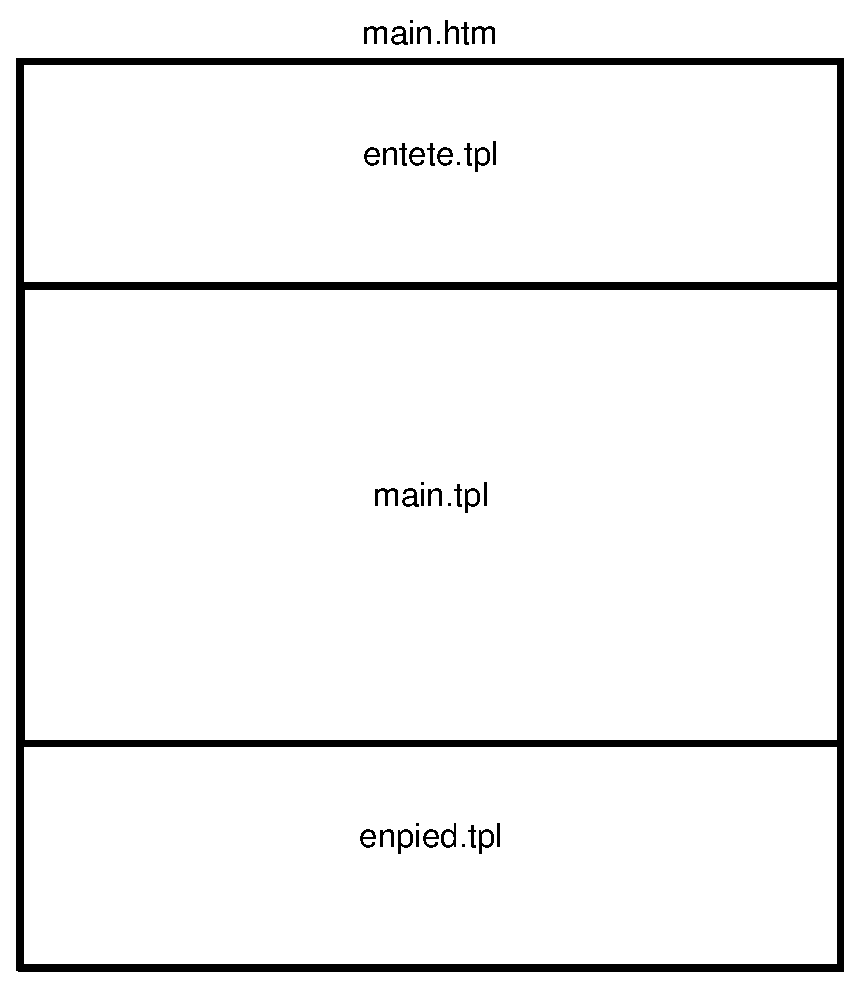
\includegraphics[width=0.7\linewidth]{dessin/templates}
\caption{}
\end{figure}

En principe, seul le modèle \textit{main.tpl} change de page en page. Il est modifié en utilisant l'assignation :
\begin{lstlisting}
$set->("nom_du_modele.tpl", "corps");
\end{lstlisting}

Un autre modèle est incorporé systématiquement : main\_js.tpl.  Il contient toutes les assignations de feuilles de style, de classes ou fonctions Javascript complémentaires utilisées dans l'application.


\subsection{Conventions de nommage}

Les templates sont stockés dans le dossier display/templates. Le dossier display/templates\_c est utilisé par Smarty pour préparer l'affichage, et doit donc être accessible en écriture au serveur web.

Pour simplfier la navigation, les templates doivent être stockés dans un sous-dossier dont le nom doit être identique au nom du sous-dossier contenant les modules PHP. Les fichiers doivent commencer par le nom du module, et se terminer par l'action correspondante, par exemple \textit{poissonList.tpl}, \textit{poissonChange.tpl}, etc. 
Cela facilite la recherche des templates en regroupant par ordre alphabétique les modèles qui portent sur le même sujet.

\section{La vue Ajax}
Nom de la classe : \textbf{VueAjaxJson}.

Elle encode le tableau fourni par la fonction \textit{set()} au format Json, et transmet la chaîne générée au navigateur, après avoir nettoyé le cache.

\section{La vue CSV}

Nom de la classe : \textbf{VueCsv}.

Fonctions disponibles : 
\begin{longtable}{|p{5cm}|p{8cm}|}
\hline
\textbf{fonction} & \textbf{Objectif} \\
\hline
\endhead
setFilename(\$filename) & indique le nom à utiliser pour générer le fichier\\
\hline
send(\$param = "") & Déclenche l'envoi du tableau vers le navigateur, au format CSV. \textit{param} peut contenir le nom du fichier souhaité. S'il est vide, le nom du fichier transmis par la fonction précédente est utilisé. Sinon, un nom de fichier, contenant la date, est généré.\\
\hline
\caption{Fonctions déclarées dans la classe VueCsv}
\end{longtable}

La fonction set() doit être utilisée pour indiquer le tableau à transformer en CSV. La classe va générer automatiquement une ligne d'entête à partir du nom des colonnes de la première ligne.

En l'état actuel, il n'est pas possible de définir des options particulières pour la génération du fichier CSV.

\section{La vue binaire}

Nom de la classe : \textbf{VueBinaire}.

Cette vue est utilisée pour envoyer des données sous forme binaire au navigateur (images, par exemple). Les données doivent avoir été auparavant générées dans un fichier du serveur web : c'est le contenu du fichier qui est transmis.

Fonctions disponibles : 
\begin{longtable}{|p{5cm}|p{8cm}|}
\hline
\textbf{fonction} & \textbf{Objectif} \\
\hline
\endhead
setParam(array \$param) & transmet un tableau contenant l'ensemble des paramètres à utiliser pour générer le fichier. Les paramètres sont les suivants : \\
& \textit{filename} : nom du fichier tel qu'il apparaîtra dans le navigateur \\
& \textit{disposition} : \textit{attachment} (fichier joint) ou \textit{inline} (affichage direct dans le navigateur) \\
& \textit{tmp\_name} : nom du fichier dans le serveur \\
& \textit{content\_type} : type mime. S'il n'est pas indiqué, le programme essaiera de le déterminer à partir du contenu du fichier \\
\hline
send() & Envoie le fichier au navigateur, en fonction des paramètres indiqués \\
\hline
\caption{Fonctions déclarées dans la classe VueBinaire}
\end{longtable}

\section{La vue PDF}

Nom de la classe : \textbf{VuePdf}.

Il s'agit d'une variante de la vue précédente. Elle accepte non pas le nom d'un fichier, mais la référence correspondant à une fonction \textit{fopen()} ou équivalente. Cette approche est nécessaire si le fichier PDF à envoyer à été stocké dans une base de données ouverte avec PDO.

Fonctions disponibles :
\begin{longtable}{|p{5cm}|p{8cm}|}
\hline
\textbf{fonction} & \textbf{Objectif} \\
\hline
\endhead

setFileReference(\$ref)& indique la référence du fichier à traiter (résultat de fopen() ou d'une lecture PDO)\\
\hline
setFilename(\$filename)& Nom du fichier tel qu'il sera transmis au navigateur. S'il n'est pas précisé, il sera généré (en cas d'attachement) \\
\hline
setDisposition(\$disp = "attachment")& Indique la manière d'envoyer le fichier au navigateur. Valeurs acceptées : \textit{attachment} ou \textit{inline}\\
\hline
send() & Envoie le fichier au navigateur, en fonction des paramètres indiqués \\
\hline
\caption{Fonctions déclarées dans la classe VuePdf}
\end{longtable}

La classe peut générer des exceptions en cas de problème.

\chapter{Génération du menu}
Pour les pages web, le menu est généré de manière dynamique :
\begin{itemize}
\item lors du premier appel à l'application ;
\item après toute opération de connexion ou de déconnexion.
\end{itemize}

Le menu est stocké en variable de session, pour accélérer l'affichage.

Il est structuré sous la forme d'une liste non ordonnée (balises \textit{ul} et \textit{li}), et contient les classes utilisées par \textit{bootstrap} pour son affichage.

\section{Fichier de description}

Le menu est généré à partir du fichier \textbf{param/menu.xml}. La branche principale s'appelle \textit{<menu>}. Voici un exemple d'entrée, qui correspond au menu d'administration :

\begin{lstlisting}
<item module="administration" label="Administration" tooltip="Administration de l'application" droits="admin">
	<item module="loginList" menulevel="1" menuorder="9" droits="admin" label="Liste des comptes locaux" tooltip="Liste des logins - identification via la base de données"/>
	<item module="appliList" droits="admin" label="ACL - droits" tooltip="applications et droits gérés"/>
	<item module="aclloginList" droits="admin" label="ACL - logins" tooltip="Logins déclarés dans le module de gestion des droits"/>
	<item module="groupList" droits="admin" label="ACL - groupes de logins" tooltip="Groupes de logins et logins rattachés aux groupes"/>
	<item module="dbparamList" droits="admin" label="Paramètres de l'application" tooltip="Liste des paramètres pérennes de l'application" />
	<item module="phpinfo" droits="admin" label="PHP info" tooltip="configuration générale du serveur PHP"/>
</item>
\end{lstlisting}

Les entrées du menu sont déclarées dans des balises \textbf{item}. Voici les attributs utilisables :

\begin{longtable}{|p{2.5cm}|c|p{9cm}|}
\hline
\textbf{Attribut} & \textbf{Requis} & \textbf{Signification} \\
\hline
\endhead
module & X & Nom du module à exécuter, tel que décrit dans le fichier actions.xml (\textit{cf.} \ref{actions} \textit{\nameref{actions}}, page \pageref{actions})\\
 \hline
droits & & Droit nécessaire pour afficher l'entrée du menu. Il est possible d'indiquer plusieurs droits, en les séparant par une virgule\\
 \hline
loginrequis & & Si vaut 1, l'entrée ne sera affichée que si l'utilisateur est connecté \\
 \hline
onlynoconnect & & Si vaut 1, l'entrée ne sera affichée que si l'utilisateur n'est pas connecté\\
 \hline
label & X & Texte affiché\\
 \hline
tooltip & X & libellé affiché au survol de la souris (attribut HTML \textit{title})\\
 \hline

\caption{Liste des attributs utilisables pour décrire les entrées du menu}
\end{longtable}

Une entrée \textit{item} peut contenir d'autres entrées \textit{item}, ce qui permet de décrire les menus en cascade. Actuellement, le menu n'a été testé qu'avec 2 niveaux (menu principal horizontal, et menus verticaux associés).

L'ordre d'affichage est celui décrit dans le fichier xml.

\section{Génération en mode développement}

Si la variable \textit{APPLI\_modeDeveloppement} est positionnée à \textit{true}, le menu est généré à chaque appel.

\chapter{Gestion des langues}\label{langue}

Le framework a été conçu pour supporter plusieurs langues européennes.

Depuis juillet 2018, il utilise la fonction \textit{gettext} pour traduire tous les libellés. La mise au point a été réalisée par Alexandre Maindron, dans le cadre du projet Collec-Science \href{https://github.com/Irstea/collec}{https://github.com/Irstea/collec}.

Les fichiers de traduction sont déclarés dans le dossier locales/C/LC\_MESSAGES. Le fichier .po contient les libellés à traduire et leur traduction, le fichier .mo la valeur compilée.

Le script \textit{generate\_translation.sh} récupère tous les libellés à traduire, lance le programme \href{https://poedit.net/}{poedit}, et compile le résultat dans le fichier .mo. Le script détaille précisément les opérations effectuées, notamment la récupération des libellés dans les fichiers xml ou dans les modèles Smarty.

Les fichiers locales/fr.php et locales/en.php ne sont plus utilisés que pour définir des paramètres généraux, notamment pour traiter les formats de dates.

\chapter{Compléments sur Smarty}\label{smarty}

\section{Syntaxe générale}
Smarty est basé sur le langage PHP : il est possible d'utiliser beaucoup de mécanismes du langage, notamment les fonctions de test.

Les commandes Smarty sont encadrées dans des accolades. L'analyseur est capable de rechercher des balises dans des chaînes encadrées par des guillemets ou des cottes. Toute commande ou ordre Smarty doit toucher l'accolade ouvrante.

Les variables, comme en PHP, doivent commencer par le caractère \textit{dollar}.

\subsection{Encadrement des libellés pour gérer le multilinguisme}

Pour qu'ils puissent être pris en charge par GETTEXT et traduits dans la langue demandée, les libellés doivent être encadrés par les balises t :
\begin{lstlisting}
{t}libellé à afficher{/t}
\end{lstlisting}

\subsection{Cohabitation Javascript et Smarty}

Les fonctions Javascript sont, elles aussi, encadrées par des accolades. Pour permettre d'insérer des variables Smarty dans du code Javascript, il suffit de respecter les règles suivantes :
\begin{itemize}
\item toute commande Smarty doit impérativement toucher l'accolade ouvrante ;
\item tout code Javascript doit être séparé de l'accolade ouvrante par un espace.
\end{itemize}

Exemple :
\begin{lstlisting}
function fonctionJavascript() {
var varJavascript = {$variableSmarty};
}
\end{lstlisting}

La variable \textit{varJavascript} sera assignée avec le contenu de la variable \textit{\$variableSmarty}, transmise par Smarty.

\subsection{Affichage d'une variable}

Une variable assignée à Smarty est affichée ainsi :

Code PHP :
\begin{lstlisting}
$vue->set("contenu","varSmarty");
\end{lstlisting}

Dans le template :
\begin{lstlisting}
{$varSmarty}
\end{lstlisting}
affichera la valeur \textit{contenu}.


\subsection{Affichage d'une liste}
En général, l'interrogation de la base de données ramène un tableau associatif, chaque ligne contient un tableau avec le nom des attributs comme clé, et la valeur de l'attribut associé.

Smarty dispose d'un mécanisme permettant de traiter un tableau facilement.

Voici d'abord le code PHP :
\begin{lstlisting} 
$vue->set($instance_objetBDD->getListe(), "data");
\end{lstlisting}

Et le code permettant de l'afficher dans le template :
\begin{lstlisting}
{section name=lst loop=$data}
{$data[lst].attr1} {$data[lst].attr2}<br>
{/section}
\end{lstlisting}

Les attributs \textit{attr1} et \textit{attr2} de toutes les lignes seront affichés les uns au dessous des autres.

\subsubsection{Dans un tableau - Datatables}

Le framework utilise le composant Datatables (\url{datatables}) pour l'affichage des tableaux. Datatables a été paramétré pour trier correctement les dates (plugin qui reconnaît automatiquement les libellés de type date).

Pour qu'une table soit reconnue comme un composant Datatables, il suffit de lui rajouter la classe datatable. Voici un exemple d'utilisation :
\begin{lstlisting}
<table id="exampleList" class="table table-bordered table-hover datatable " >
<thead>
<tr>
<th>Date</th>
<th>Comments</th>
<th>status</th>
</tr>
</thead><tbody>
{section name=lst loop=$data}
<tr>
<td>
{if $droits["gestion"] == 1}
<a href="index.php?module=exampleChange&example_id={$data[lst].example_id}">
{$data[lst].example_date}
</a>
{else}
{$data[lst].example_date}
{/if}
</td>
<td>{$data[lst].comment}</td>
<td><span class="textareaDisplay">{$data[lst].example_comment}</span></td>
</tr>
{/section}
</tbody>
</table>
{/if}
\end{lstlisting}

Chaque ligne du corps est traité dans la section. Cet exemple rajoute en plus l'accès à la page de modification, selon les droits définis (\textit{cf.} \ref{droits} \textit{\nameref{droits}}, page \pageref{droits}).

Pour modifier l'ordre de tri ou d'autres paramètres du composant Datatables, le plus simple est de rajouter ce code après l'affichage du tableau :

\begin{lstlisting}
$(document).ready(function() {
	var exempleList = $("#exempleList").DataTable();
	exempleList.order([[1, 'desc'], [0, 'desc']]).draw();
});
</script>
\end{lstlisting}

L'ordre des colonnes commence à 0.

\subsubsection{Dans un select}

Dans les formulaires, des champs de type \textit{select} est souvent utilisé pour proposer une liste fermée de choix à l'utilisateur. 

Voici comment l'implémenter dans un template :

\begin{lstlisting}
<select id="container_type_id" name="container_type_id" class="form-control">
<option value="" {if $data.container_type_id == ""}selected{/if}>Selectionnez...</option>
{section name=lst loop=$container_type}
<option value="{$container_type[lst].container_type_id}" {if $container_type[lst].container_type_id == $data.container_type_id}selected{/if}>
{$container_type[lst].container_type_name}
</option>
{/section}
</select>
\end{lstlisting}

Dans cet exemple, le champ container\_container\_id doit être sélectionné à partir de la liste contenue dans \textit{container\_type}. Ici, l'utilisateur peut ne pas renseigner l'information : la première option peut être vide. Si le champ doit être obligatoire, il suffit de supprimer la première option.

Des tests sont réalisés pour positionner correctement l'indicateur \textit{selected} lors de l'affichage en modification.

\subsection{Les tests}

Les tests sont classiques, sous la forme : 
\begin{lstlisting}
{if condition_de_test}

{else}

{/if}
\end{lstlisting}

Les conditions de test sont celles de PHP, par exemple :
\begin{lstlisting}
{if strlen($variable) > 0}
...
{/if}
\end{lstlisting}

\subsection{Les variables internes}
Les sections disposent de variables permettant de connaître le nombre d'occurrences d'un tableau, l'occurrence courante... Avec des composants comme Datatables, on ne les utilise guère.

Par contre, il est parfois nécessaire de réaliser quelques calculs : il est possible d'assigner des variables facilement (le code a été simplifié par rapport aux premières versions) :

\begin{lstlisting}
{$variable = 0}
{$section name=lst loop=$data}
{$variable = $variable + $data[lst].montant}
{/section}
Montant total : {$variable}
\end{lstlisting}

\section{Affichage des libellés en fonction de la langue}

Comme nous l'avons vu précédemment (\textit{cf.} \ref{langue} \textit{\nameref{langue}}, page \pageref{langue}), les libellés sont stockés dans la variable \$LANG. Il est alors assez facile de les afficher dans le template. Voici un exemple correspondant à l'affichage du libellé \textit{Rechercher} :
\begin{lstlisting}
<button name="{$LANG[message].21}>
\end{lstlisting}


\section{Organisation des formulaires de saisie}

En raison du parti-pris du framework de séparer toutes les actions et de pouvoir leur imposer des droits différents, la gestion d'un formulaire de saisie est un peu compliquée. À partir du même formulaire, il faut pouvoir aussi bien déclencher l'écriture d'une information (\textit{write}) que supprimer l'enregistrement (\textit{delete}). 

Il est possible de gérer deux formulaires différents, l'un étant dédié uniquement au bouton \textit{Supprimer}. L'approche actuelle est plutôt d'utiliser du javascript pou générer automatiquement l'action correspondante.

Voici un exemple de formulaire implémentant ce fonctionnement :

\begin{lstlisting}
<form class="form-horizontal protoform" id="exampleForm" method="post" action="index.php">
<input type="hidden" name="example_id" value="{$data.example_id}">
<input type="hidden" name="moduleBase" value="example">
<input type="hidden" name="action" value="Write">

<div class="form-group center">
      <button type="submit" class="btn btn-primary button-valid">{$LANG["message"].19}</button>
      {if $data.example_id > 0 }
      <button class="btn btn-danger button-delete">{$LANG["message"].20}</button>
      {/if}
 </div>
</form>
\end{lstlisting}

Le formulaire doit comprendre la classe \textit{protoform}, et deux champs cachés : \textit{moduleBase} et \textit{action}. Les boutons doivent être des classes \textit{button-valid} ou \textit{button-delete}, pour respectivement déclencher l'écriture ou la suppression de l'enregistrement.

Le code Javascript associé (déjà déclaré dans le framework) va permettre de modifier le contenu du champ \textit{action} si le bouton \textit{Supprimer} est actionné. Le contrôleur reconstituera le module demandé en associant les deux champs.

\part{Sécurité et implémentation}
\chapter{Mécanismes de sécurité et mise en production}

\section{Protections générales}
\subsection{Durée de la session}
Par défaut, les sessions ont une durée de vie d'une heure sans activité. Elles sont supprimées automatiquement, sans tenir compte le cas échéant du cookie de session. Ce dernier est transmis en \textit{http\_only} et en mode \textit{secure}.

Si la session dure plus d'une heure\footnote{la durée par défaut de la session}, l'identifiant de session est régénéré.

\subsection{Protection contre le changement d'adresse IP}

Si l'adresse IP du client change pendant la session, celle-ci est fermée. L'adresse IP récupérée tient compte, le cas échéant, d'un passage par un serveur \textit{Reverse-Proxy}.

\section{Intégrer le transcodage des clés}

Dans certains cas de figure, l'utilisateur ne peut traiter que certains enregistrements d'une table. Le framework dispose d'une classe qui permet de transcoder les clés, pour éviter que l'on puisse modifier indûment une clé.

la classe \textit{TranslateId} (fichier \textit{framework/translateId/translateId.class.php}) permet de gérer le transcodage des clés.

Cette classe doit être instanciée en variable de session.

\subsection{Charger le fichier de classe avant le démarrage de la session}

Dans \textit{modules/beforesession.inc.php}, rajoutez la ligne suivante :
\begin{lstlisting}
require_once 'framework/translateId.translateId.class.php';
\end{lstlisting}

\subsection{Instancier la classe}
Voici un exemple d'instanciation :
\begin{lstlisting}
if (!isset($_SESSION["ti_table"]) 
	$_SESSION["ti_table"] = new TranslateId("id");
\end{lstlisting}

\textit{id} correspond au nom de la colonne à transcoder.



\chapter{Mise en production}

\section{Configuration et installation générale}

\subsection{Configuration du serveur web}

\subsection{Nettoyage de l'application et contrôles à réaliser}

\subsection{Installation de la base de données des droits}

\subsection{Nettoyage des comptes par défaut}

\section{Travailler avec plusieurs applications différentes à partir du même code}\label{dnsmultiple}

Dans certains cas, l'application réalisée doit permettre de travailler avec des bases de données différentes selon le contexte, pour éviter de mélanger les informations. La première solution consiste à créer autant de copies que nécessaire du logiciel.

La seconde consiste à n'utiliser qu'un seul code, mais en paramétrant les informations spécifiques à chaque base de données.

Voici le principe général (\textit{cf.} schéma \ref{dnsmultipleschema})  :
\begin{figure}[th]
\label{dnsmultipleschema}
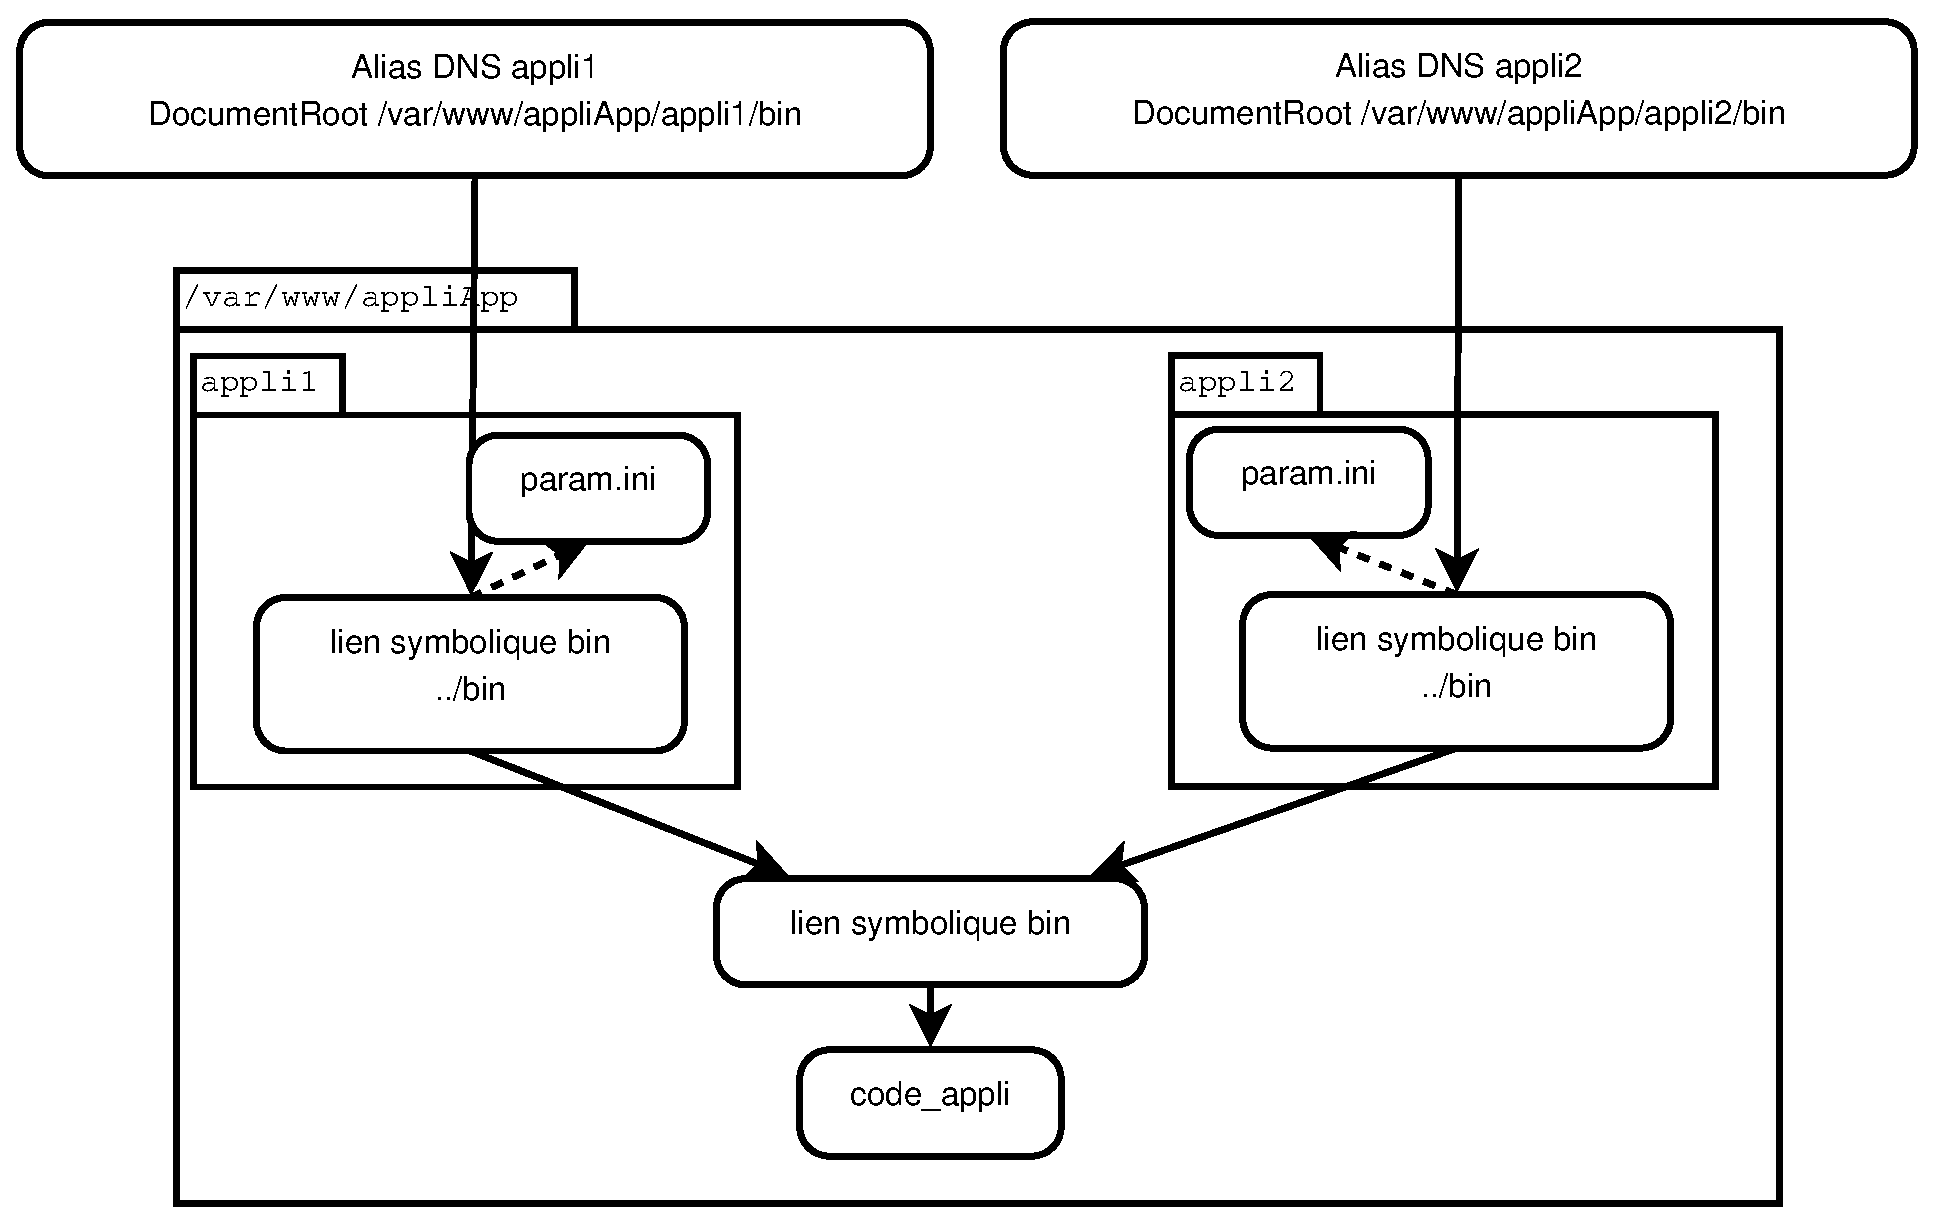
\includegraphics[width=\linewidth]{dessin/dnsmultiple}
\caption{Schéma général d'implémentation pour utiliser le même code avec des noms d'application et des jeux de données différents}
\end{figure}

Dans le paramétrage de l'alias DNS (en principe, dans \textbf{/etc/apache2/sites-available}), l'application pointe vers le dossier \textbf{/var/www/appliApp/appli1/bin}. 
\textit{/var/www} correspond à la racine du site web, \textit{appliApp} au dossier racine de l'application, \textit{appli1} au dossier spécifique de l'alias DNS.

Ce dossier \textit{appli1} ne contient que deux fichiers : \textbf{param.ini}, qui contient les paramètres spécifiques, et \textbf{bin}, qui est un lien symbolique vers le dossier \textbf{../bin}. 

Le dossier \textit{../bin} (donc, dans \textit{/var/www/appliApp}) est lui aussi un alias qui pointe vers le code réel de l'application, ici \textbf{code\_appli}.

Le fichier \textbf{param.inc.php} décrit l'entrée suivante :
\begin{lstlisting}
$paramIniFile = "../param.ini";
\end{lstlisting}

Le fichier \textbf{param.ini} sera cherché dans le dossier parent du code de l'application, c'est à dire soit dans \textit{appli1}, soit dans \textit{appli2} dans cet exemple.

Il suffit qu'il contienne les paramètres adéquats pour rendre l'application utilisable dans des contextes différents à partir du même code initial.

\end{document}